\chapter{A interação humano--computacional em ação: uma aplicação \textit{web} interativa}


Discutimos até aqui fundamentos teóricos dos algoritmos, análises de complexidade, resultados empíricos e princípios pedagógicos que justificam o uso de ferramentas interativas. Estabelecemos \emph{o quê} ensinar (Chu–Liu/Edmonds e Frank), \emph{por quê} usar visualizações (redução de carga cognitiva, dual coding, engajamento ativo) e \emph{como} estruturar o design (heurísticas de IHC, visão geral com detalhe sob demanda, feedback imediato).


Agora, traduzimos esses princípios em código e interface: a aplicação \textit{web} que desenvolvemos busca materializar cada uma das diretrizes discutidas. Isto é, cada botão, cada visualização e cada mensagem de log foi projetada intencionalmente, guiada pelos princípios de IHC e pelas necessidades pedagógicas identificadas.


A aplicação \textit{web} interativa foi desenvolvida para ilustrar os algoritmos de Chu–Liu/Edmonds e Frank, permitindo aos usuários acompanhar passo a passo o funcionamento de ambos os métodos. A ferramenta foi projetada com base em princípios de interação humano-computador, visando maximizar a compreensão e o engajamento dos usuários.

\section{Princípios de interação humano-computador}


A interação humano-computador (IHC) estuda como projetar sistemas computacionais que sejam eficientes, eficazes e agradáveis para os usuários.


Sintetizando heurísticas de usabilidade e descoberta \cite{nielsen1994heuristics,shneiderman2016designing} e quadros de interação e aprendizagem \cite{rogers2011interaction,mayer2009multimedia,sweller1988cognitive,naps2003engagement}, destacamos oito princípios orientadores: (i) usabilidade, (ii) eficiência cognitiva, (iii) feedback imediato, (iv) engajamento ativo, (v) visão geral com detalhe sob demanda (mantra \emph{overview→filter→details} de \cite{shneiderman1996eyes}), (vi) consistência semântica, (vii) múltiplos registros de representação e (viii) prevenção/recuperação de erros. A seguir descrevemos cada um e sua materialização na ferramenta.


\subsection{Usabilidade}

Usabilidade refere-se à facilidade com que os usuários podem aprender a usar um sistema, realizar tarefas e alcançar seus objetivos. Na nossa aplicação, priorizamos uma interface limpa e intuitiva, com controles claros para navegar pelos passos dos algoritmos, selecionar arestas, visualizar cortes ativos e entender a evolução dos custos reduzidos.

\subsection{Eficiência cognitiva}

Eficiência cognitiva envolve minimizar a carga cognitiva dos usuários, facilitando a compreensão e o processamento de informações. Implementamos visualizações que destacam mudanças importantes (como contrações e expansões) e fornecem explicações textuais concisas para cada passo, ajudando os usuários a conectar ações com conceitos teóricos.

\subsection{Feedback Imediato}

Feedback imediato é crucial para manter os usuários informados sobre o estado do sistema e as consequências de suas ações. Nossa ferramenta oferece feedback visual e textual em tempo real, mostrando como cada ação afeta o grafo e os custos associados, reforçando a compreensão causal.

\subsection{Engajamento ativo}

Engajamento ativo refere-se à participação dos usuários no processo de aprendizagem, incentivando-os a explorar, experimentar e interagir com o sistema. Nossa aplicação promove o engajamento ativo ao permitir que os usuários manipulem o grafo, testem diferentes abordagens e visualizem os resultados de suas ações em tempo real.


\subsection{Visão geral com detalhe sob demanda}

A visão geral com detalhe sob demanda permite que os usuários obtenham uma compreensão ampla do sistema, enquanto ainda têm acesso a informações detalhadas quando necessário. Implementamos essa abordagem ao fornecer uma visualização geral do grafo, com a opção de expandir informações sobre arestas e nós específicos conforme o interesse do usuário.

\subsection{Consistência semântica}

A consistência semântica garante que os elementos da interface e suas interações sejam compreensíveis e previsíveis. Nossa ferramenta mantém a consistência semântica ao usar terminologia e representações visuais padronizadas em toda a aplicação, facilitando a compreensão dos usuários.

\subsection{Múltiplos registros de representação}

Múltiplos registros de representação referem-se à capacidade de apresentar informações de diferentes maneiras, atendendo às preferências e estilos de aprendizagem dos usuários. Nossa aplicação oferece várias representações do grafo (visual, textual, interativa), permitindo que os usuários escolham a forma que melhor se adapta às suas necessidades.

\subsection{Prevenção de erros}

A prevenção de erros envolve projetar o sistema de forma a minimizar a probabilidade de erros dos usuários. Implementamos medidas de prevenção de erros, como validação de entrada e feedback em tempo real, para ajudar os usuários a evitar ações indesejadas e compreender melhor as consequências de suas escolhas.


Esses princípios de interação humano-computador foram fundamentais para o desenvolvimento da nossa aplicação \textit{web} interativa, garantindo que ela seja não apenas funcional, mas também acessível e eficaz como ferramenta de aprendizagem. A seguir, detalhamos a implementação técnica da aplicação e como ela se posiciona no ecossistema de ferramentas didáticas para o ensino de grafos.

\begin{table}[H]
	\centering
	\renewcommand{\arraystretch}{1.18}
	\setlength{\tabcolsep}{6pt}
	\footnotesize
	% Ajuste de larguras: 1a coluna ampliada para evitar overlap; leve redução na 3a.
	\begin{tabular}{p{2.9cm} p{4.0cm} p{7.0cm}}
		\hline
		\textbf{Princípio}                               & \textbf{Exemplo Geral}                         & \textbf{Materialização na Aplicação}                                                                                                                                            \\
		\hline
		Usabilidade                                      & Botões claros para avançar/voltar etapas       & Barra de controles com rótulos diretos (Adicionar Aresta, Executar, Reset); agrupamento visual consistente via Tailwind; nenhum menu profundo aninhado.                         \\
		Eficiência\newline cognitiva                     & Reduzir elementos irrelevantes no estado atual & Layout estável entre passos; apenas arestas relevantes destacadas; eliminação de ornamentação visual; custos e rótulos legíveis sem rotação.                                    \\
		Feedback\newline imediato                        & Mostrar efeito de uma ação logo após o clique  & Cada ação dispara: (i) atualização do desenho do grafo, (ii) entrada no log textual explicando a mudança (ex.: contração, seleção de aresta).                                   \\
		Engajamento\newline ativo                        & Usuário prediz antes de revelar próximo passo  & Controles passo a passo permitem explorar sequencialmente; usuário insere/edita pesos e escolhe raiz antes de rodar o algoritmo.                                                \\
		Visão geral→\newline Detalhes                    & Visão global com acesso a informação pontual   & Visão completa do grafo em todos os passos + possibilidade de inspecionar pesos e arestas específicas no log sequencial; estados anteriores preservados para comparação mental. \\
		Consistência\newline semântica                   & Mesmo conceito, mesma cor/forma                & Raiz destacada de forma fixa; arestas selecionadas mantêm estilo; semântica cromática não muda entre passos (evita remapeamento mental).                                        \\
		Múltiplos\newline registros                      & Texto + grafo + (futuro) estrutura derivada    & Combinação de: descrição textual no log, representação visual do grafo, parâmetros simbólicos (pesos); prepara expansão futura para mostrar custos reduzidos.                   \\
		Prevenção /\newline recuperação\newline de erros & Impedir entrada inválida / ação reversível     & Validação de pesos (numéricos); bloqueio de execução sem raiz definida; botão Reset para recompor estado limpo sem recarregar página.                                           \\
		\hline
	\end{tabular}
	\caption{Síntese dos princípios de interação humano-computador aplicados e sua realização concreta na ferramenta interativa.}
	\label{tab:principios-ihc}
\end{table}

\section{Descrição da aplicação}

A aplicação \textit{web} interativa foi desenvolvida para ilustrar os algoritmos de Chu–Liu/Edmonds e Frank, permitindo aos usuários acompanhar passo a passo o funcionamento de ambos os métodos. A ferramenta foi projetada com base em princípios de interação humano-computador, visando maximizar a compreensão e o engajamento dos usuários.


\subsection{Visão geral das páginas}
A aplicação \textit{web} é composta por páginas HTML autônomas carregadas no navegador, cada uma focada em um aspecto: (i) \texttt{home.html} (apresentação / resumo), (ii) \texttt{chuliu.html} (execução passo a passo do algoritmo de Chu--Liu/Edmonds), (iii) \texttt{andrasfrank.html} (estrutura para futura visualização da abordagem primal--dual), (iv) \texttt{draw\_graph.html} (editor livre de grafos), além do componente compartilhado de navegação lateral \texttt{sidebar.html}. Cada página injeta o \texttt{sidebar} dinamicamente e carrega scripts específicos.

\subsection{Bibliotecas e dependências}


O desenvolvimento utilizou tecnologias \textit{web} modernas, incluindo HTML5, Tailwind CSS para estilos responsivos, e PyScript para execução de código Python diretamente no navegador. A biblioteca NetworkX foi empregada para manipulação de grafos, enquanto Matplotlib gerou visualizações estáticas dos estados intermediários. O código foi estruturado para modularidade e clareza, facilitando futuras extensões. Detalhamos abaixo esses aspectos:

\begin{itemize}\setlength{\itemsep}{2pt}
	\item \textbf{Frontend:} HTML5 + Tailwind CSS para composição responsiva e estilos utilitários consistentes.
	\item \textbf{Execução Python no cliente:} PyScript (carregado via CDN) provê execução de módulos Python (ex.: \texttt{networkx}, \texttt{matplotlib}) sem instalação local, reduzindo barreira de entrada didática.
	\item \textbf{Bibliotecas centrais:} NetworkX para manipulação de grafos dirigidos; \texttt{matplotlib} para renderização de snapshots; (em páginas avançadas) Cytoscape.js previsto para interação rica (estrutura já importada em \texttt{chuliu.html} / \texttt{andrasfrank.html}).
	\item \textbf{Empacotamento de estado:} Serialização JSON (formato \texttt{node\_link}) para exportação e reuso analítico.
	\item \textbf{Isolamento:} Cada página carrega apenas os elementos necessários, evitando \emph{payload} excessivo e minimizando latência de interface (princípio de eficiência cognitiva).
\end{itemize}

\subsection{Componentes funcionais principais}

A aplicação centraliza-se nas páginas \texttt{chuliu.html} e \texttt{andrasfrank.html}, que permitem executar os algoritmos de Chu--Liu/Edmonds e Frank, respectivamente. A seguir, detalhamos os componentes funcionais principais da interface:

\begin{enumerate}\setlength{\itemsep}{2pt}
	\item \textbf{Editor de Grafo:} inputs para origem, destino e peso + botões de inserção e limpeza (\texttt{add-edge}, \texttt{reset-graph}).
	\item \textbf{Carregamento de exemplo:} botão \texttt{load-test-graph} injeta um grafo de teste estruturado para reduzir \emph{time-to-first-insight}.
	\item \textbf{Configuração de raiz:} campo para definir / confirmar o vértice raiz (\texttt{root-node}).
	\item \textbf{Execução algorítmica:} botão \texttt{run-algorithm} dispara o pipeline de filtragem e cálculo da arborescência mínima.
	\item \textbf{Visualização de estados:} área cumulativa (\texttt{graph-area}) onde cada renderização mantém a coerência posicional (layout determinístico) para comparação mental entre passos.
	\item \textbf{Log textual:} caixa de texto incremental (\texttt{log-output}) correlaciona ações a transformações estruturais (dual coding: texto + imagem).
	\item \textbf{Exportação:} ação de exportar grafo em JSON para análise posterior ou reimportação.
	\item \textbf{Incorporação de PDF:} \texttt{tese.html} exibe o \texttt{main.pdf} lado a lado à aplicação, incentivando leitura entrelaçada teoria-execução.
\end{enumerate}

\subsection{Fluxo de interação}

O fluxo de interação foi projetado para ser linear e intuitivo, guiando o usuário desde a criação do grafo até a visualização dos resultados do algoritmo. A seguir, descrevemos o fluxo típico:

\begin{enumerate}\setlength{\itemsep}{2pt}
	\item Usuário monta ou carrega um grafo de teste.
	\item Define (ou confirma) o vértice raiz \(r_0\).
	\item Executa o algoritmo (Chu--Liu/Edmonds): são aplicadas normalizações e seleção de arestas (implementação apresentada em seções anteriores / listagens).
	\item Observa estados sequenciais: cada snapshot reforça invariantes (arestas escolhidas, pesos, estrutura alcançada).
	\item (Opcional) Exporta o grafo resultante para replicação em notebooks ou comparação com a abordagem dual futura.
\end{enumerate}

\subsection{Estado e dados persistentes}

O estado principal é mantido em memória (objeto \texttt{networkx.DiGraph}). O log textual funciona como uma \emph{trilha de auditoria didática}. Cada ação do usuário (adição de aresta, definição de raiz, execução de passo) atualiza o grafo e o log, permitindo rastrear a evolução do estado. A exportação em JSON facilita a reimportação e análise posterior.

\subsection{Limitações atuais}

Atualmente, a aplicação apresenta algumas limitações que podem impactar a experiência do usuário e a eficácia da visualização:

\begin{itemize}\setlength{\itemsep}{2pt}
	\item Ausência de visualização explícita de contração de ciclos (marcação diferenciada por cores/aglomerados ainda não implementada).
	\item Não há comparação lado a lado (split view) entre algoritmos (Chu--Liu vs. Frank) ainda.
	\item Layout planar simples pode falhar em instâncias mais densas (sobreposição de rótulos) — futura substituição por \texttt{spring} ou \texttt{dagre}-like adaptativo.
	\item Falta camada de destaque cromático para custos reduzidos e arcos “apertados” \((c' = 0)\).
	\item Exportação limita-se ao grafo final; não há pacote de estados intermediários (\emph{replay}).
\end{itemize}

\subsection{Melhorias futuras}

Desse modo, entendemos que a aplicação, embora funcional, pode ser aprimorada com recursos adicionais para enriquecer a experiência didática. Algumas melhorias incluem:

\begin{itemize}\setlength{\itemsep}{2pt}
	\item Visualização animada da contração/reexpansão de ciclos com agrupamento colapsável.
	\item Camada de coloração para arestas com custo reduzido zero e cortes ativos.
	\item Geração automática de relatório (log + estados selecionados) em PDF/ZIP.
	\item Módulo paralelo para a abordagem primal--dual de Frank (empacotamento de cortes e duas fases).
	\item Modo “comparativo” exibindo diferenças de passos e métricas agregadas.
	\item Instrumentação de métricas (tempo por passo, número de contrações, distribuição de pesos normalizados).
\end{itemize}


De modo geral, a aplicação serve como um protótipo funcional que demonstra o potencial de ferramentas interativas para o ensino de algoritmos complexos em teoria dos grafos. Com melhorias contínuas, pode se tornar uma plataforma robusta para aprendizagem ativa e visualização didática. Na seção seguinte, detalhamos aspectos técnicos da implementação.

\section{Detalhes de Implementação}

A aplicação foi implementada utilizando tecnologias \textit{web} modernas, com foco em simplicidade, modularidade e reprodutibilidade. A seguir, detalhamos os principais aspectos técnicos da implementação.

\subsection{Estrutura de arquivos}

A estrutura de arquivos da aplicação é organizada da seguinte forma:
\begin{itemize}\setlength{\itemsep}{2pt}
	\item \texttt{main.py}: script Python principal contendo funções de manipulação de grafos e lógica algorítmica.
	\item \texttt{index.html}: página inicial com resumo e links para outras seções.
	\item \texttt{chuliu.html}: página dedicada à execução do algoritmo de Chu--Liu/Edmonds.
	\item \texttt{andrasfrank.html}: página para futura implementação do algoritmo de Frank.
	\item \texttt{draw\_graph.html}: editor livre de grafos.
	\item \texttt{sidebar.html}: componente de navegação lateral compartilhado.
	\item \texttt{styles.css}: arquivo de estilos customizados (além do Tailwind).
	\item \texttt{scripts/}: diretório contendo scripts Python e JavaScript.
	\item \texttt{assets/}: diretório para imagens, ícones e outros recursos estáticos.
\end{itemize}

\subsection{Códigos principais}

A seguir, apresentamos os códigos desenvolvidos para os algoritmos implementados realizarem a interação com os usuários.

\subsection{\texttt{Main.py}:} o arquivo \texttt{main.py} contém funções para manipulação de grafos, execução dos algoritmos e geração de visualizações.


As funções principais incluem:
\begin{itemize}\setlength{\itemsep}{2pt}
	\item \texttt{draw\_graph(G, title, append)}: renderiza o grafo \(G\) com título e opção de anexar ou substituir a visualização.
	\item \texttt{add\_edge()}: adiciona uma aresta ao grafo com base nos inputs do usuário.
	\item \texttt{reset\_graph()}: limpa o grafo atual e o log.
	\item \texttt{export\_graph()}: exporta o grafo atual em formato JSON.
	\item \texttt{load\_test\_graph()}: carrega um grafo de teste predefinido.
	\item \texttt{run\_algorithm()}: executa o algoritmo de Chu--Liu/Edmonds, aplicando filtragem e visualizando cada passo.
\end{itemize}

A seguir, apresentamos essas funções conforme implementadas no arquivo \texttt{main.py}.

\begin{pybox}[label={lst:draw_graph}]{Main.py: manipulação e visualização de grafos}
	import networkx as nx
	from networkx.readwrite import json_graph
	import matplotlib.pyplot as plt
	from js import Blob, URL, document, alert
	from pyscript import when, display
	import json

	from chuliu import find_optimum_arborescence_chuliu, remove_edges_to_r0

	def log_in_box(msg: str):
	log_box = document.getElementById("log-output")
	log_box.value += msg + "\n"
	log_box.scrollTop = log_box.scrollHeight

	def draw_graph(G: nx.DiGraph, title="Digrafo", append=True):
	plt.clf()  # Limpa a figura atual
	pos = nx.planar_layout(G)  # Layout para posicionamento dos nós
	plt.figure(figsize=(6, 4))  # Tamanho da figura
	# Desenha os nós e arestas
	nx.draw(
	G,
	pos,
	with_labels=True,
	node_color="lightblue",
	edge_color="gray",
	node_size=2000,
	font_size=12,
	)
	weights = nx.get_edge_attributes(G, "w")
	nx.draw_networkx_edge_labels(
	G, pos, edge_labels=weights, font_color="red", font_size=12
	)
	plt.title(title)
	display(title, target="graph-area", append=append)
	display(plt, target="graph-area", append=append)
	plt.close()  # Fecha a figura para liberar memória

	G = nx.DiGraph()

	@when("click", "#add-edge")
	def add_edge():
	global G
	source = document.getElementById("source").value
	target = document.getElementById("target").value
	weight = document.getElementById("weight").value
	if source and target and weight:
	G.add_edge(source, target, w=float(weight))
	log_in_box(f"Aresta adicionada: {source} → {target} (peso={weight})")
	draw_graph(G, "Grafo com Arestas", append=False)

	@when("click", "#reset-graph")
	def reset_graph():
	global G
	G.clear()
	document.getElementById("log-output").value = ""
	draw_graph(G, "Grafo Resetado", append=False)
	log_in_box("Grafo resetado.")

	@when("click", "#export-graph")
	def export_graph(event):
	log_in_box("Exportando grafo...")
	global G
	if G.number_of_nodes() == 0:
	log_in_box("[ERRO] O grafo está vazio.")
	return

	# Converte o grafo para JSON
	data = json_graph.node_link_data(G, edges="links")
	json_data = json.dumps(data, indent=4)

	# Cria um link de download no navegador
	blob = Blob.new([json_data], {"type": "application/json"})
	url = URL.createObjectURL(blob)

	# Configura e dispara o download
	link = document.createElement("a")
	link.href = url
	link.download = "graph_teste.json"
	link.click()
	URL.revokeObjectURL(url)

	log_in_box("Download do grafo iniciado.")

	@when("click", "#load-test-graph")
	def load_test_graph(event):
	global G
	G.clear()
	G.add_edge("r0", "B", w=10)
	G.add_edge("r0", "A", w=2)
	G.add_edge("r0", "C", w=10)
	G.add_edge("B", "A", w=1)
	G.add_edge("A", "C", w=4)
	G.add_edge("C", "D", w=2)
	G.add_edge("D", "B", w=2)
	G.add_edge("B", "E", w=8)
	G.add_edge("C", "E", w=4)

	log_in_box("Grafo de teste carregado.")
	draw_graph(G, "Grafo de Teste (DG)", append=False)

	@when("click", "#show-ready-arborescence")
	def show_ready_arborescence(event):
	T = nx.DiGraph()
	T.add_edge("r0", "A", w=2)
	T.add_edge("A", "C", w=4)
	T.add_edge("C", "D", w=2)
	T.add_edge("D", "B", w=2)
	T.add_edge("C", "E", w=4)
	draw_graph(T, "Arborescência Pré-definida")
	log_in_box("Arborescência pronta exibida.")


	@when("click", "#run-algorithm")
	def run_algorithm(event):
	global G
	r0 = document.getElementById("root-node").value or "r0"
	if r0 not in G:
	alert(f"[ERRO] O nó raiz '{r0}' deve existir no grafo.")
	return

	log_in_box("Executando algoritmo de Chu-Liu...")
	print(remove_edges_to_r0)
	G_filtered = remove_edges_to_r0(G, r0)
	T = find_optimum_arborescence_chuliu(
	G_filtered, r0, draw_fn=draw_graph, log=log_in_box
	)
	draw_graph(T, "Arborescência Ótima")
	log_in_box("Execução concluída com sucesso.")
\end{pybox}

\subsection{\texttt{Index.html}:} o arquivo \texttt{index.html} define a estrutura principal da página HTML, incluindo a integração com PyScript e Tailwind CSS para estilos responsivos. A seguir, apresentamos o código completo dessa página.

\begin{htmlbox}[label={lst:index_html}]{Estrutura principal da página HTML com PyScript}
	<!DOCTYPE html>
	<html>
	<head>
	<meta charset="utf-8" />
	<meta name="viewport" content="width=device-width,initial-scale=1" />
	<title>Chu-Liu/Edmonds Visualizer</title>
	<script src="https://cdn.tailwindcss.com"></script>
	<link
	rel="stylesheet"
	href="https://pyscript.net/releases/2025.3.1/core.css"
	/>
	<script
	type="module"
	src="https://pyscript.net/releases/2025.3.1/core.js"
	></script>
	</head>
	<body class="bg-gray-100">
	<header class="bg-[#5b8f79] text-white text-center p-6">
	<h1 class="text-3xl font-bold">Chu-Liu/Edmonds Visualizer</h1>
	<p class="text-lg mt-2">
	Visualização passo a passo de arborescências em grafos direcionados
	</p>
	</header>

	<main class="flex flex-col items-center gap-8 py-8 px-8">
	<section class="text-center w-full max-w-4xl">
	<h2 class="text-2xl font-semibold text-[#5b8f79] mb-4">
	Definir Di-grafo
	</h2>
	<div class="flex flex-wrap justify-center gap-4 items-center mb-4">
	<input
	type="text"
	id="source"
	placeholder="Origem"
	class="p-3 border rounded border-gray-300 w-40"
	/>
	<input
	type="text"
	id="target"
	placeholder="Destino"
	class="p-3 border rounded border-gray-300 w-40"
	/>
	<input
	type="number"
	id="weight"
	placeholder="Peso"
	min="0"
	class="p-3 border rounded border-gray-300 w-40"
	/>
	<button
	id="add-edge"
	class="p-3 bg-[#5b8f79] text-white font-bold rounded hover:bg-[#4a7a66]"
	>
	Adicionar Aresta
	</button>
	</div>
	<div class="flex flex-wrap justify-center gap-4 items-center mb-4">
	<button
	id="reset-graph"
	class="p-3 bg-[#5b8f79] text-white font-bold rounded hover:bg-[#4a7a66]"
	>
	Limpar Grafo
	</button>
	<button
	id="export-graph"
	class="p-3 bg-[#5b8f79] text-white font-bold rounded hover:bg-[#4a7a66]"
	>
	Exportar Grafo para JSON
	</button>
	</div>
	<div class="flex flex-wrap justify-center gap-4 items-center mb-4">
	<button
	id="load-test-graph"
	class="p-3 bg-[#5b8f79] text-white font-bold rounded hover:bg-[#4a7a66]"
	>
	Carregar Grafo de Teste
	</button>
	<button
	id="show-ready-arborescence"
	class="p-3 bg-[#5b8f79] text-white font-bold rounded hover:bg-[#4a7a66]"
	>
	Mostrar Arborescência do Grafo de Teste
	</button>
	</div>
	</section>

	<section class="text-center w-full max-w-4xl">
	<h2 class="text-2xl font-semibold text-[#5b8f79] mb-4">
	Executar Algoritmo de Chu-Liu/Edmonds
	</h2>
	<div class="flex flex-wrap justify-center gap-4 items-center">
	<label for="root-node" class="text-gray-700 font-medium"
	>Nó Raiz:</label
	>
	<input
	type="text"
	id="root-node"
	placeholder="Nó Raiz"
	value="r0"
	class="p-3 border rounded border-gray-300 w-40"
	/>
	<button
	id="run-algorithm"
	class="p-3 bg-[#5b8f79] text-white font-bold rounded hover:bg-[#4a7a66]"
	>
	Executar Algoritmo
	</button>
	</div>
	</section>

	<section
	id="graph-output"
	class="w-full max-w-4xl bg-white p-6 rounded shadow"
	>
	<h2 class="text-2xl font-semibold text-[#5b8f79] mb-4">Grafo Atual</h2>
	<py-script id="graph-area"></py-script>
	</section>

	<section id="log" class="w-full max-w-4xl bg-white p-6 rounded shadow">
	<h2 class="text-2xl font-semibold text-[#5b8f79] mb-4">
	Log da Execução
	</h2>
	<textarea
	id="log-output"
	readonly
	class="w-full p-3 border rounded border-gray-300 h-40"
	></textarea>
	</section>
	</main>

	<script type="py" src="./main.py" config="./pyscript.json"></script>
	</body>
	</html>
\end{htmlbox}


\subsection{Demais Páginas da Aplicação \textit{web}}
Além da página principal do visualizador, a aplicação inclui um conjunto de páginas modulares que suportam a navegação e fornecem contexto adicional. A seguir, detalhamos a estrutura e função de cada uma dessas páginas.

\subsection{\texttt{Home.html}:} o arquivo \texttt{home.html} serve como a página inicial da aplicação, oferecendo uma visão geral do projeto, incluindo um resumo do trabalho e informações sobre os integrantes. A estrutura da página é projetada para ser acolhedora e informativa, utilizando Tailwind CSS para garantir uma aparência moderna e responsiva. Abaixo, apresentamos um exemplo de captura de tela da página.

% Screenshot da página Home
\begin{figure}[H]\centering
	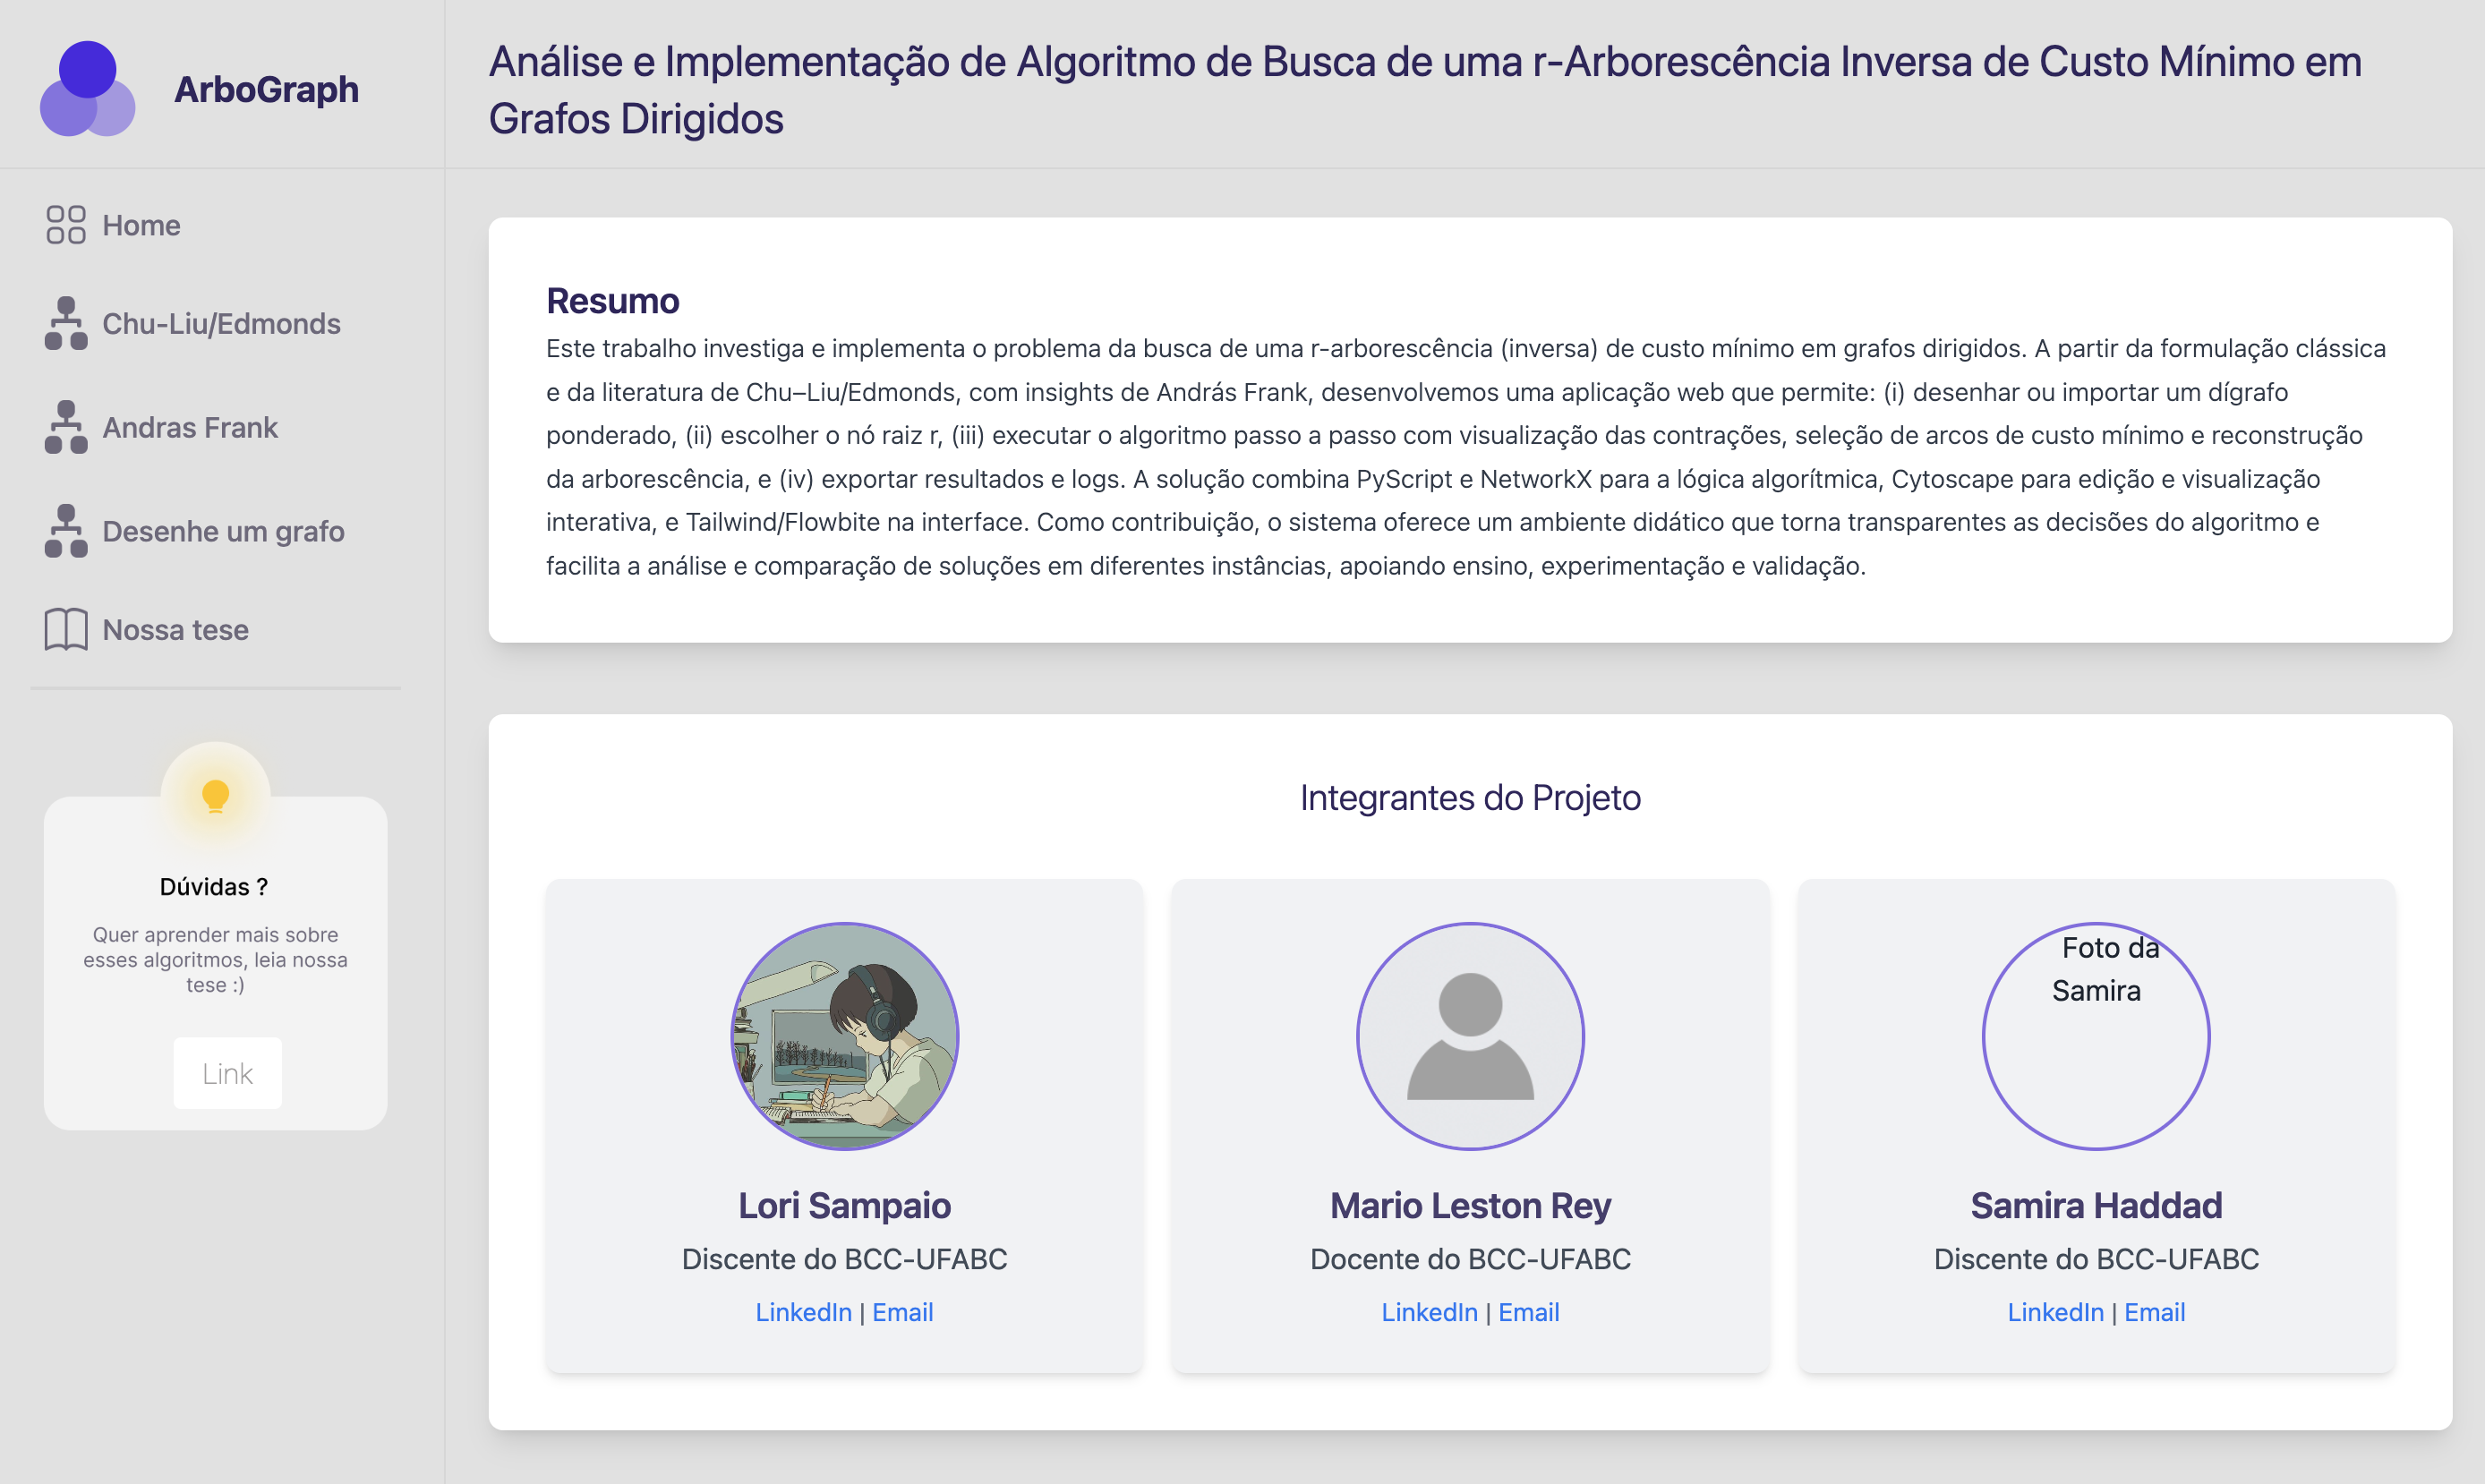
\includegraphics[width=0.95\textwidth]{../assets/homehtml.png}
	\caption{Captura de tela de \texttt{home.html}: visão geral com resumo e integrantes.}
	\label{fig:home_html_screenshot}
\end{figure}


A seguir, apresentamos o código completo dessa página.

\begin{htmlbox}{home.html}
	<!DOCTYPE html>
	<html lang="pt-BR">

	<head>
	<meta charset="UTF-8" />
	<meta name="viewport" content="width=device-width, initial-scale=1" />
	<title>Arbograph</title>
	<link rel="icon" type="image/x-icon" href="../assets/logo.png"/>
	<script src="https://cdn.tailwindcss.com"></script>
	<link rel="stylesheet" href="https://pyscript.net/releases/2025.3.1/core.css" />
	<script type="module" src="https://pyscript.net/releases/2025.3.1/core.js"></script>
	</head>

	<body class="flex min-h-screen text-gray-800 bg-gray-100">
	<style>
	.py-error,
	.py-terminal-error {
	display: none !important;
	}
	</style>
	<div class="absolute top-[100px] w-full h-[1px] bg-[#DBDBDB]"></div>

	<!-- MENU LATERAL -->
	<div id="sidebar"></div>

	<!-- CONTEÚDO PRINCIPAL -->
	<div id="main-content" class="flex-1 bg-[#E5E5E5] p-6">
	<!-- Análise e Implementação de Algoritmo de Busca de uma r-Arborescência Inversa de Custo Mínimo em Grafos Dirigidos -->
	<span class="flex items-center gap-4 mb-10 text-2xl text-[#352B67]">Análise e Implementação de Algoritmo de Busca de uma r-Arborescência Inversa de Custo Mínimo em Grafos Dirigidos</span>
	<section class="mb-10 bg-white p-8 rounded-lg shadow-lg" id="resumo">
	<scan class="text-3xl font-semibold text-center mb-8 text-[#352B67] text-xl">Resumo</scan>
	<div class="prose max-w-none text-gray-700">
	<scan class="text-lg leading-relaxed mb-4 text-sm font-light">
	At vero eos et accusamus et iusto odio dignissimos ducimus qui
	blanditiis praesentium voluptatum deleniti atque corrupti quos
	dolores et quas molestias excepturi sint occaecati cupiditate non
	provident, similique sunt in culpa qui officia deserunt mollitia a
	nimi, id est laborum et dolorum fuga. Et harum quidem rerum facilis
	est et expedita distinctio. Nam libero tempore, cum soluta nobis est eligendi
	optio cumque nihil impedit quo minus id quod maxime placeat facere possimus, omnis voluptas
	assumenda est, omnis dolor repellendus. Temporibus autem quibusdam et aut officiis debitis aut
	rerum necessitatibus saepe eveniet ut et voluptates repudiandae sint et molestiae non recusandae.
	Itaque earum rerum hic tenetur a sapiente delectus, ut aut reiciendis voluptatibus maiores alias .
	</scan>
	</div>
	</section>
	<section class="bg-white p-8 rounded-lg shadow-lg" id="integrantes">
	<h2 class="text-3xl font-light text-center mb-8 text-[#352B67] text-xl">Integrantes do Projeto</h2>

	<div class="grid grid-cols-1 md:grid-cols-3 lg:grid-cols-3 gap-4 justify-items-center">
	<div class="bg-gray-100 p-6 rounded-lg shadow-md text-center flex flex-col items-center w-full max-w-sm">
	<img src="../assets/lori.jpg" alt="Foto da Lori"
	class="w-32 h-32 rounded-full object-cover mb-4 border-2 border-[#8d79e5]">
	<h3 class="text-xl font-semibold text-[#4f4678]">Lori Sampaio</h3>
	<p class="text-gray-600 mt-1">Discente do BCC-UFABC</p>
	<p class="text-sm text-gray-500 mt-2">
	<a href="https://linkedin.com/in/integrante1" target="_blank"
	class="text-blue-500 hover:underline">LinkedIn</a> |
	<a href="mailto:lorenypsum@gmail.com" class="text-blue-500 hover:underline">Email</a>
	</p>
	</div>
	<div class="bg-gray-100 p-6 rounded-lg shadow-md text-center flex flex-col items-center w-full max-w-sm">
	<img src="https://www.ufabc.edu.br/images/conteudo/img-padrao-autor.png" alt="Foto do Mario"
	class="w-32 h-32 rounded-full object-cover mb-4 border-2 border-[#8d79e5]">
	<h3 class="text-xl font-semibold text-[#4f4678]">Mario Leston Rey</h3>
	<p class="text-gray-600 mt-1">Docente do BCC-UFABC</p>
	<p class="text-sm text-gray-500 mt-2">
	<a href="#" target="_blank"
	class="text-blue-500 hover:underline">LinkedIn</a> |
	<a href="mailto:mario.leston@ufabc.edu.br" class="text-blue-500 hover:underline">Email</a>
	</p>
	</div>
	<div class="bg-gray-100 p-6 rounded-lg shadow-md text-center flex flex-col items-center w-full max-w-sm">
	<img src="https://media.licdn.com/dms/image/v2/C4D03AQHr9O4LzxUomQ/profile-displayphoto-shrink_400_400/profile-displayphoto-shrink_400_400/0/1646342924520?e=1753920000&v=beta&t=8fpR8VQiVYX_2xWaQwUXK6NqxKbHVYvGKH1ProxHogg" alt="Foto da Samira"
	class="w-32 h-32 rounded-full object-cover mb-4 border-2 border-[#8d79e5]">
	<h3 class="text-xl font-semibold text-[#4f4678]">Samira Haddad</h3>
	<p class="text-gray-600 mt-1">Discente do BCC-UFABC</p>
	<p class="text-sm text-gray-500 mt-2">
	<a href="https://www.linkedin.com/in/samirahad" target="_blank"
	class="text-blue-500 hover:underline">LinkedIn</a> |
	<a href="mailto:samira.had.2000@gmail.com" class="text-blue-500 hover:underline">Email</a>
	</p>
	</div>


	</div>
	</section>
	</div>

	<!-- Scripts -->
	<script src="../scripts/js/sidebar.js"></script>
	<script src="../scripts/js/main.js"></script>
	</body>
	</html>
\end{htmlbox}


\begin{figure}[H]\centering
	\begin{tikzpicture}[>=Stealth, node distance=1.8cm]
		\node[draw,rounded corners,fill=gray!10] (sb) {Sidebar};
		\node[draw,rounded corners,fill=blue!10,right=3cm of sb,minimum width=5cm,minimum height=2cm] (mc) {Main Content};
		\node[draw,fill=white,rounded corners,below=0.2cm of mc,minimum width=4cm] (res) {Resumo};
		\node[draw,fill=white,rounded corners,below=0.2cm of res,minimum width=4cm] (int) {Integrantes};
		\draw[->] (res) -- (int);
	\end{tikzpicture}
	\caption{\texttt{home.html}: navegação lateral + conteúdo hierárquico (contexto \textrightarrow resumo \textrightarrow equipe).}
\end{figure}
\textit{Comentário:} estrutura linear vertical facilita \emph{progressive disclosure}; separação lateral reduz interferência visual com conteúdo principal.

\subsection{\texttt{Draw\_graph.html}:} editor de grafos livre com funcionalidades de criação, edição, importação e exportação. Utiliza \texttt{Cytoscape.js} para visualização interativa e \texttt{PyScript} para lógica algorítmica. Abaixo, apresentamos uma captura de tela da página.

% Screenshot da página Draw Graph
\begin{figure}[H]\centering
	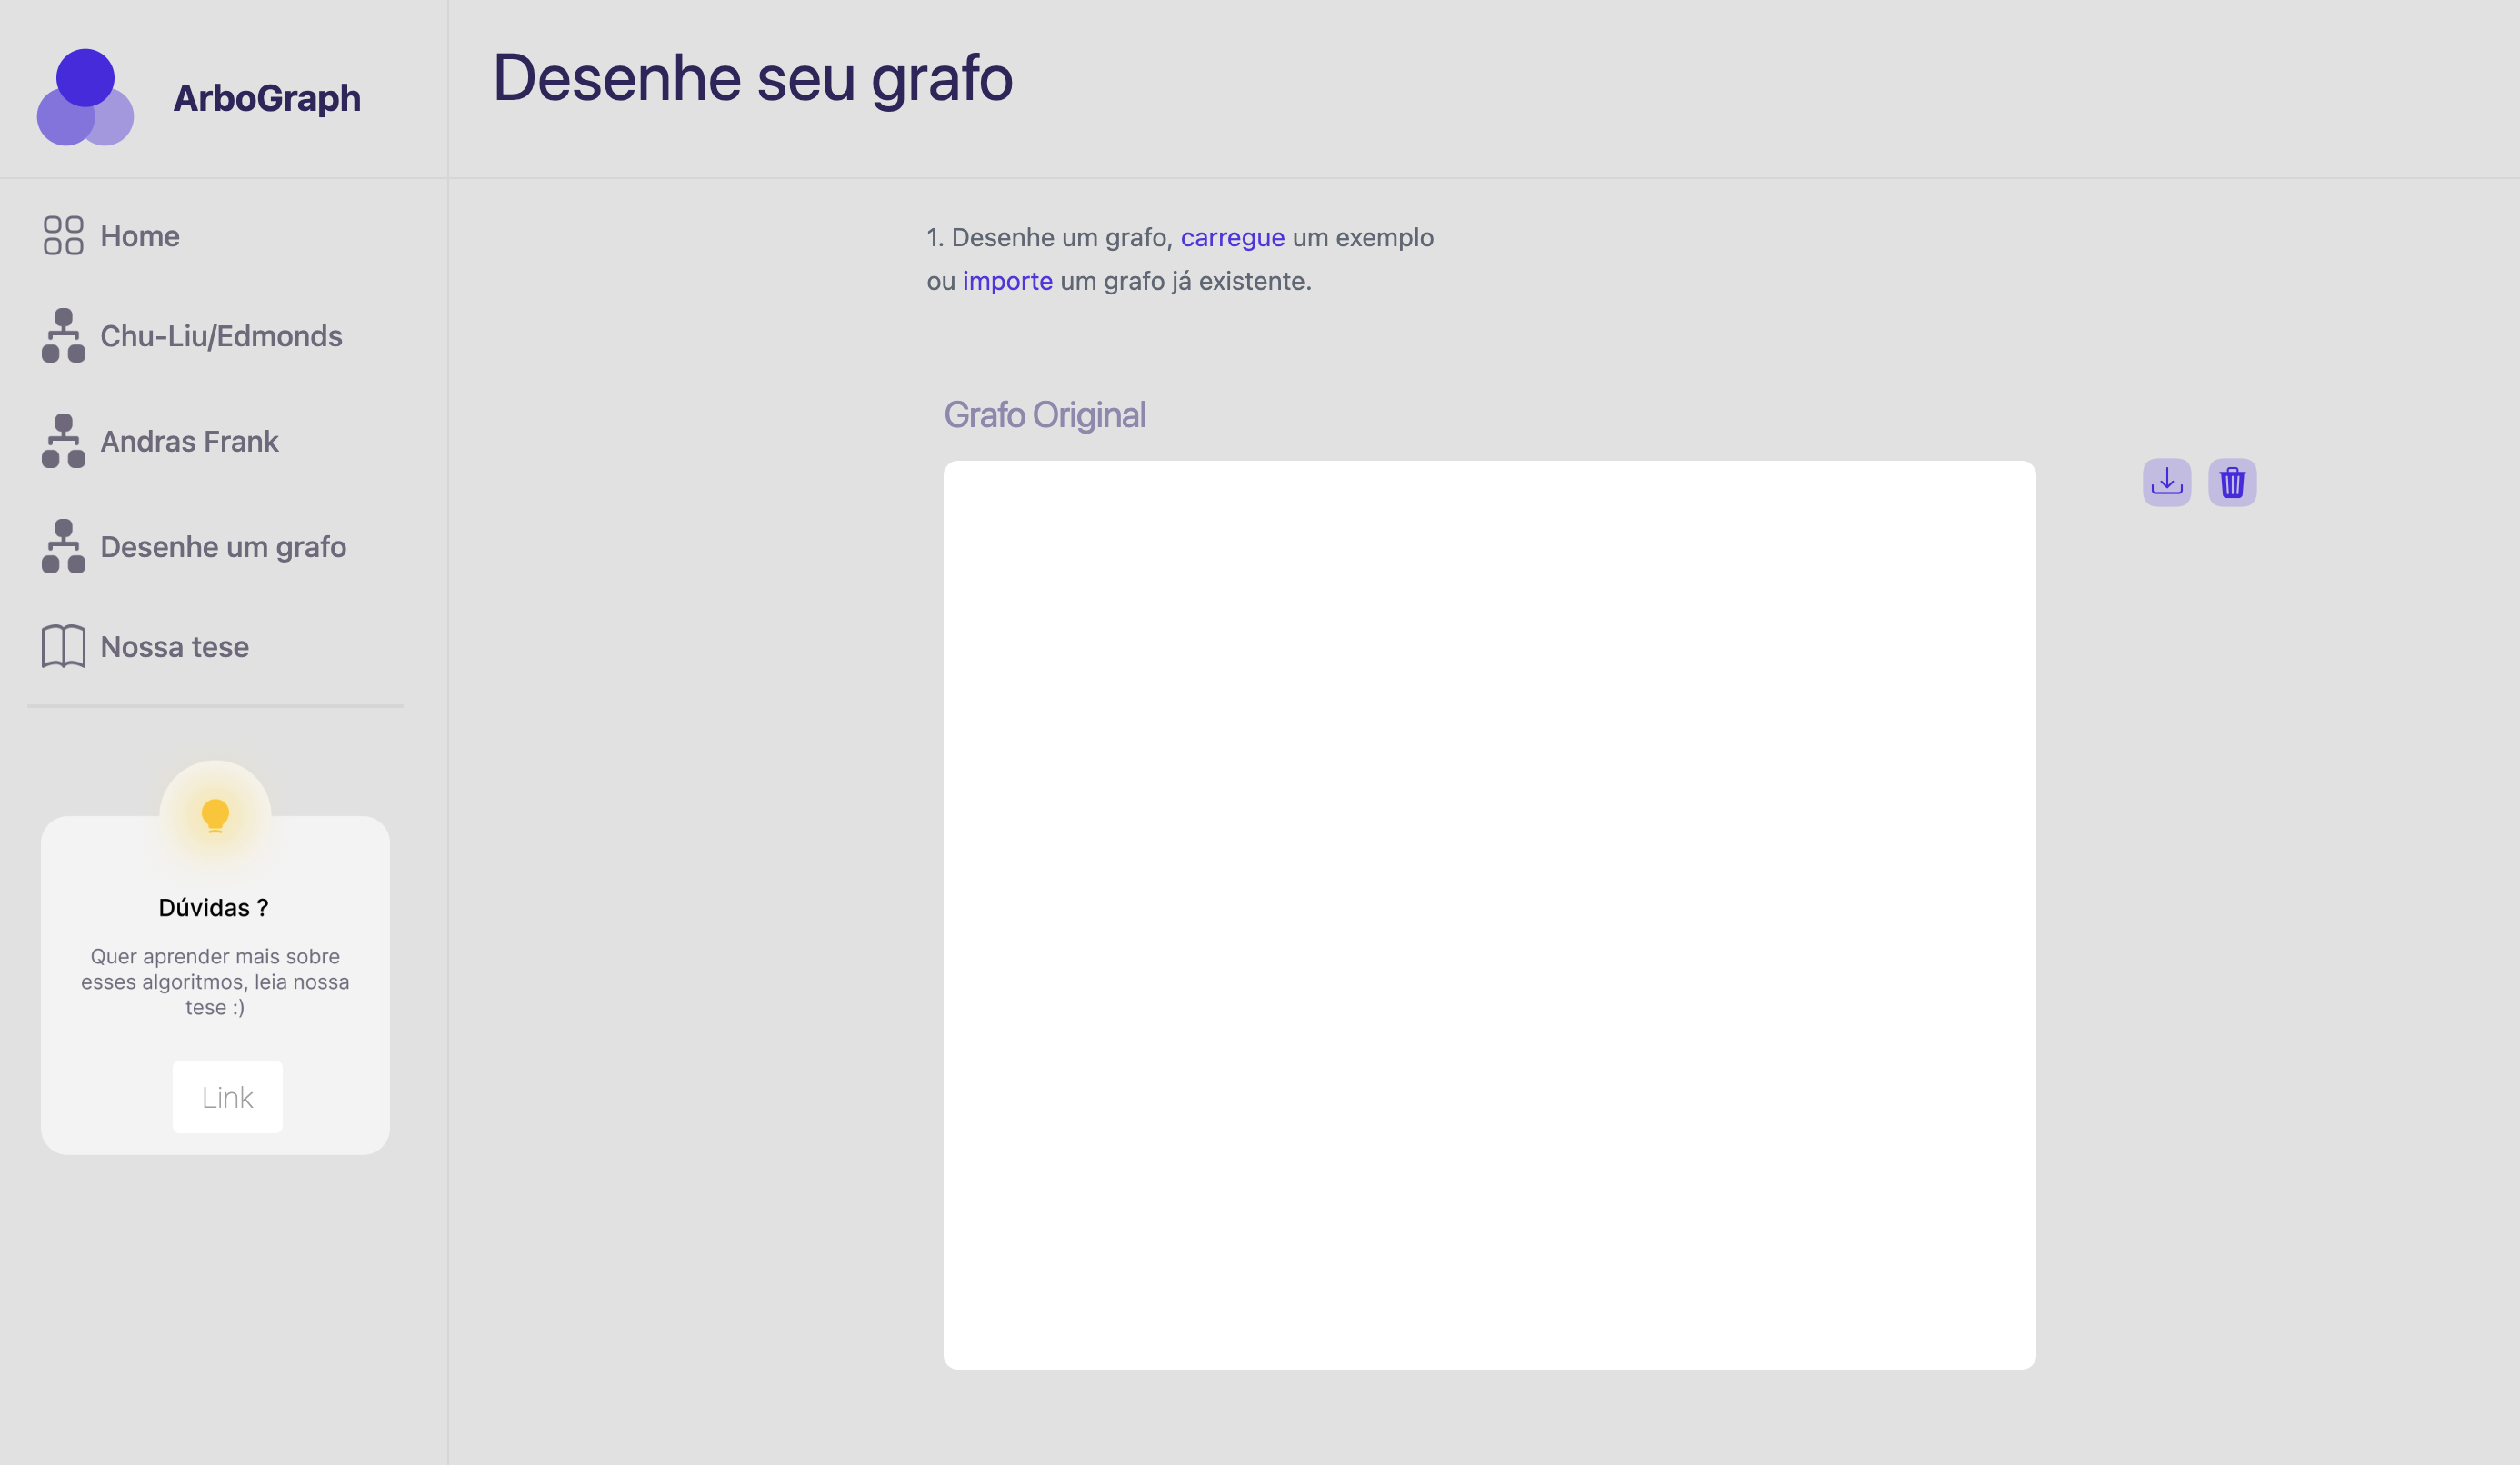
\includegraphics[width=0.95\textwidth]{../assets/drawhtml.png}
	\caption{Captura de tela de \texttt{draw\_graph.html}: editor livre de grafos.}
	\label{fig:draw_html_screenshot}
\end{figure}

A seguir, apresentamos o código completo dessa página.
\begin{htmlbox}{draw\_graph.html}
	<!DOCTYPE html>
	<html lang="pt-BR">

	<head>
	<meta charset="UTF-8" />
	<meta name="viewport" content="width=device-width, initial-scale=1" />
	<title>Desenhe seu grafo</title>
	<link rel="icon" type="image/x-icon" href="../assets/logo.png"/>
	<script src="https://cdn.tailwindcss.com"></script>
	<script src="https://unpkg.com/cytoscape@3.26.0/dist/cytoscape.min.js"></script>

	<link href="https://cdnjs.cloudflare.com/ajax/libs/flowbite/2.2.1/flowbite.min.css" rel="stylesheet" />
	<script src="https://cdnjs.cloudflare.com/ajax/libs/flowbite/2.2.1/flowbite.min.js"></script>

	<link rel="stylesheet" href="https://pyscript.net/releases/2025.3.1/core.css" />
	<script type="module" src="https://pyscript.net/releases/2025.3.1/core.js"></script>
	</head>

	<body class="flex min-h-screen text-gray-800 bg-gray-100">
	<style>
	.py-error, .py-terminal-error {
	display: none !important;
	}
	</style>
	<div class="absolute top-[100px] w-full h-[1px] bg-[#DBDBDB]"></div>

	<!-- MENU LATERAL -->
	<div id="sidebar"></div>

	<!-- CONTEÚDO PRINCIPAL -->
	<div id="main-content" class="flex-1 bg-[#E5E5E5] p-6">
	<span class="flex items-center gap-4 mb-10 text-4xl text-[#352B67]">Desenhe seu grafo</span>
	<!-- Inputs -->
	<div class="w-full flex justify-center">
	<div class="grid grid-cols-10 gap-4 w-full mx-auto">
	<div class="col-span-2 p-4"></div>
	<!-- Coluna 1 -->
	<div class="col-span-3 p-4">
	<span class="text-sm text-gray-500">
	1. Desenhe um grafo,
	<span id="load-test-graph" class="cursor-pointer text-[#5A3CE5] hover:underline">carregue</span>
	um exemplo ou
	<span id="import-graph" class="cursor-pointer text-[#5A3CE5] hover:underline">importe</span>
	<input type="file" id="file-input" style="display: none;" />
	um grafo já existente.
	</span>
	</div>
	</div>
	</div>


	<!-- Grafo original -->
	<div class="grid grid-cols-10 gap-4 py-4 px-4">
	<div class="col-span-2 p-4"></div>
	<div class="col-span-6 p-4">
	<span class="mb-50 text-xl text-[#9993B7]">Grafo Original</span>
	<div id="graph-editor" class="my-3 mt-50 py-4 px-50 rounded-lg bg-white h-[500px]">

	</div>
	</div>
	<div class="col-span-2 p-4">
	<div class="py-4 px-2 flex justify-left items-center gap-1">
	<img src="../assets/download.png" alt="Download" id="export-graph-original"
	class="my-5 cursor-pointer w-8 h-8 rounded-lg hover:opacity-80" />
	<img src="../assets/delete.png" alt="Reset" id="reset-graph"
	class="my-5 cursor-pointer w-8 h-8 rounded-lg hover:opacity-80" />
	</div>
	</div>

	</div>
	</div>

	<div id="toast-danger" class="hidden fixed top-5 right-5 z-50 flex items-center w-full max-w-xs p-4 mb-4 text-gray-500 bg-white rounded-lg shadow-sm dark:text-gray-400 dark:bg-gray-800 transition-opacity duration-500 opacity-100" role="alert">
	<div class="inline-flex items-center justify-center shrink-0 w-8 h-8 text-red-500 bg-red-100 rounded-lg dark:bg-red-800 dark:text-red-200">
	<!-- SVG de erro -->
	<svg class="w-5 h-5" aria-hidden="true" fill="currentColor" viewBox="0 0 20 20">
	<path d="M10 .5a9.5 9.5 0 1 0 9.5 9.5A9.51 9.51 0 0 0 10 .5Zm3.707 11.793a1 1 0 1 1-1.414 1.414L10 11.414l-2.293 2.293a1 1 0 0 1-1.414-1.414L8.586 10 6.293 7.707a1 1 0 0 1 1.414-1.414L10 8.586l2.293-2.293a1 1 0 0 1 1.414 1.414L11.414 10l2.293 2.293Z"/>
	</svg>
	<span class="sr-only">Error icon</span>
	</div>
	<div id="toast-danger-msg" class="ms-3 text-sm font-normal">Ocorreu um erro.</div>
	<button type="button" class="ms-auto -mx-1.5 -my-1.5 bg-white text-gray-400 hover:text-gray-900 rounded-lg focus:ring-2 focus:ring-gray-300 p-1.5 hover:bg-gray-100 inline-flex items-center justify-center h-8 w-8 dark:text-gray-500 dark:hover:text-white dark:bg-gray-800 dark:hover:bg-gray-700" data-dismiss-target="#toast-danger" aria-label="Close" onclick="document.getElementById('toast-danger').classList.add('hidden')">
	<span class="sr-only">Close</span>
	<svg class="w-3 h-3" aria-hidden="true" fill="none" viewBox="0 0 14 14">
	<path stroke="currentColor" stroke-linecap="round" stroke-linejoin="round" stroke-width="2" d="m1 1 6 6m0 0 6 6M7 7l6-6M7 7l-6 6"/>
	</svg>
	</button>
	</div>

	<!-- Scripts -->
	<script src="../scripts/js/sidebar.js"></script>
	<script src="../scripts/js/main.js"></script>
	<script src="../scripts/js/draw_graph.js"></script>
	<script type="py" src="../scripts/draw_page.py" config="../scripts/pyscript.json"></script>
	</body>
	</html>
\end{htmlbox}


A figura a seguir destaca o foco primordial no componente editor de grafos.

\begin{figure}[H]\centering
	\begin{tikzpicture}[node distance=1.2cm]
		\node[draw,rounded corners,fill=gray!10] (sb3) {Sidebar};
		\node[draw,rounded corners,fill=white,right=3cm of sb3,minimum width=6cm,minimum height=2.2cm] (ed) {Editor de Grafo};
		\node[draw,rounded corners,fill=white,below=0.2cm of ed,minimum width=3.6cm] (act) {Ações};
		\draw[->] (act) -- (ed);
	\end{tikzpicture}
	\caption{\texttt{draw\_graph.html}: foco primordial no componente editor.}
\end{figure}
\textit{Comentário:} a estrutura modular permite fácil adaptação e reutilização de componentes.

\subsection{\texttt{Sidebar.html}:} componente de navegação lateral consistente em todas as páginas. Utiliza Tailwind CSS para estilo e inclui links para as principais seções do site, reforçando um modelo mental estável de navegação. A seguir, apresentamos o código completo desse componente.

\begin{htmlbox}{sidebar.html}
	<script src="https://cdn.tailwindcss.com"></script>
	<!-- <aside class="w-64 bg-[#E5E5E5] text-white p-6 flex flex-col justify-between h-full"> -->
	<aside class="w-64 bg-[#E5E5E5] text-white p-6 flex flex-col justify-between h-full border-r-[1px] border-[#DBDBDB]">
	<div>
	<a href="home.html" class="flex items-center gap-4 mb-6 text-white font-bold text-xl">
	<img src="../assets/logo.png" alt="ArboGraph" class="w-16 h-auto" />
	<span class="text-[#352B67]">ArboGraph</span>
	</a>
	<!-- <div class="border-t-2 border-[#DBDBDB] w-full my-4"></div> -->
	<nav class="flex flex-col gap-3 text-left text-white font-medium">
	<a href="home.html" class="hover:bg-[#e0dede] p-2 rounded flex items-center gap-2">
	<img src="../assets/home.png" alt="Home" class="w-6 h-6" />
	<span class="text-[#787486]">Home</span>
	</a>
	<a href="chuliu.html" class="hover:bg-[#e0dede] p-2 rounded flex items-center gap-2">
	<img src="../assets/graph.png" alt="Chu-Liu" class="w-6" />
	<span class="text-[#787486]">Chu-Liu/Edmonds</span>
	</a>
	<a href="andrasfrank.html" class="hover:bg-[#e0dede] p-2 rounded flex items-center gap-2">
	<img src="../assets/graph.png" alt="Fulkerson" class="w-6" />
	<span class="text-[#787486]">Andras Frank</span>
	</a>
	<a href="draw_graph.html" class="hover:bg-[#e0dede] p-2 rounded flex items-center gap-2">
	<img src="../assets/graph.png" alt="Draw" class="w-6" />
	<span class="text-[#787486]">Desenhe um grafo</span>
	</a>
	<a href="tese.html" class="hover:bg-[#e0dede] p-2 rounded flex items-center gap-2">
	<img src="../assets/book.png" alt="Tesis" class="w-6 h-6" />
	<span class="text-[#787486]">Nossa tese</span>
	</a>
	<div class="border-t-[2px] border-[#DBDBDB]"></div>

	<a href="tese.html" class="relative flex items-center gap-2 mb-7 text-x">
	<img
	src="../assets/help.png"
	alt="help"
	class="w-48 mb-7 mx-auto"
	/>
	<button
	class="absolute left-20 bottom-10 bg-[#ffffff] text-[#aba9a9] font-thin py-2 px-4 rounded hover:bg-[#e0dede]"
	> Link
	</button>
	</a>
	</nav>
	</div>
	</aside>
\end{htmlbox}

A figura a seguir ilustra a estrutura hierárquica linear do menu lateral.

\begin{figure}[H]\centering
	\begin{tikzpicture}[node distance=0.9cm]
		% Ordem vertical: Home -> Chu-Liu -> Andras Frank -> Draw
		\node[draw,rounded corners,fill=gray!15,minimum width=3cm] (h) {Home};
		\node[draw,rounded corners,fill=gray!15,below=of h,minimum width=3cm] (cl) {Chu-Liu/Edmonds};
		\node[draw,rounded corners,fill=gray!15,below=of cl,minimum width=3cm] (af) {Andras Frank};
		\node[draw,rounded corners,fill=gray!15,below=of af,minimum width=3cm] (dg) {Draw};
		\node[draw,rounded corners,fill=gray!15,below=of dg,minimum width=3cm] (ts) {Tese};
		% Seta indicando hierarquia linear
		\foreach \x/\y in {h/cl,cl/af,af/dg,dg/ts} {\draw[->] (\x.south) -- (\y.north);}
	\end{tikzpicture}
	\caption{\texttt{sidebar.html}: lista vertical reforçando modelo mental estável de navegação.}
\end{figure}
\textit{Comentário:} a consistência visual e funcional do menu lateral em todas as páginas reduz a carga cognitiva associada à navegação, permitindo que os usuários se concentrem no conteúdo principal.

\subsection{\texttt{Chuliu.html}:} página dedicada ao visualizador do algoritmo de Chu-Liu/Edmonds. Inclui um passo a passo guiado para criar um grafo, selecionar o nó raiz e executar o algoritmo, com feedback visual e textual. Abaixo, apresentamos uma captura de tela da página.

% Screenshot da página Chu-Liu/Edmonds
\begin{figure}[H]\centering
	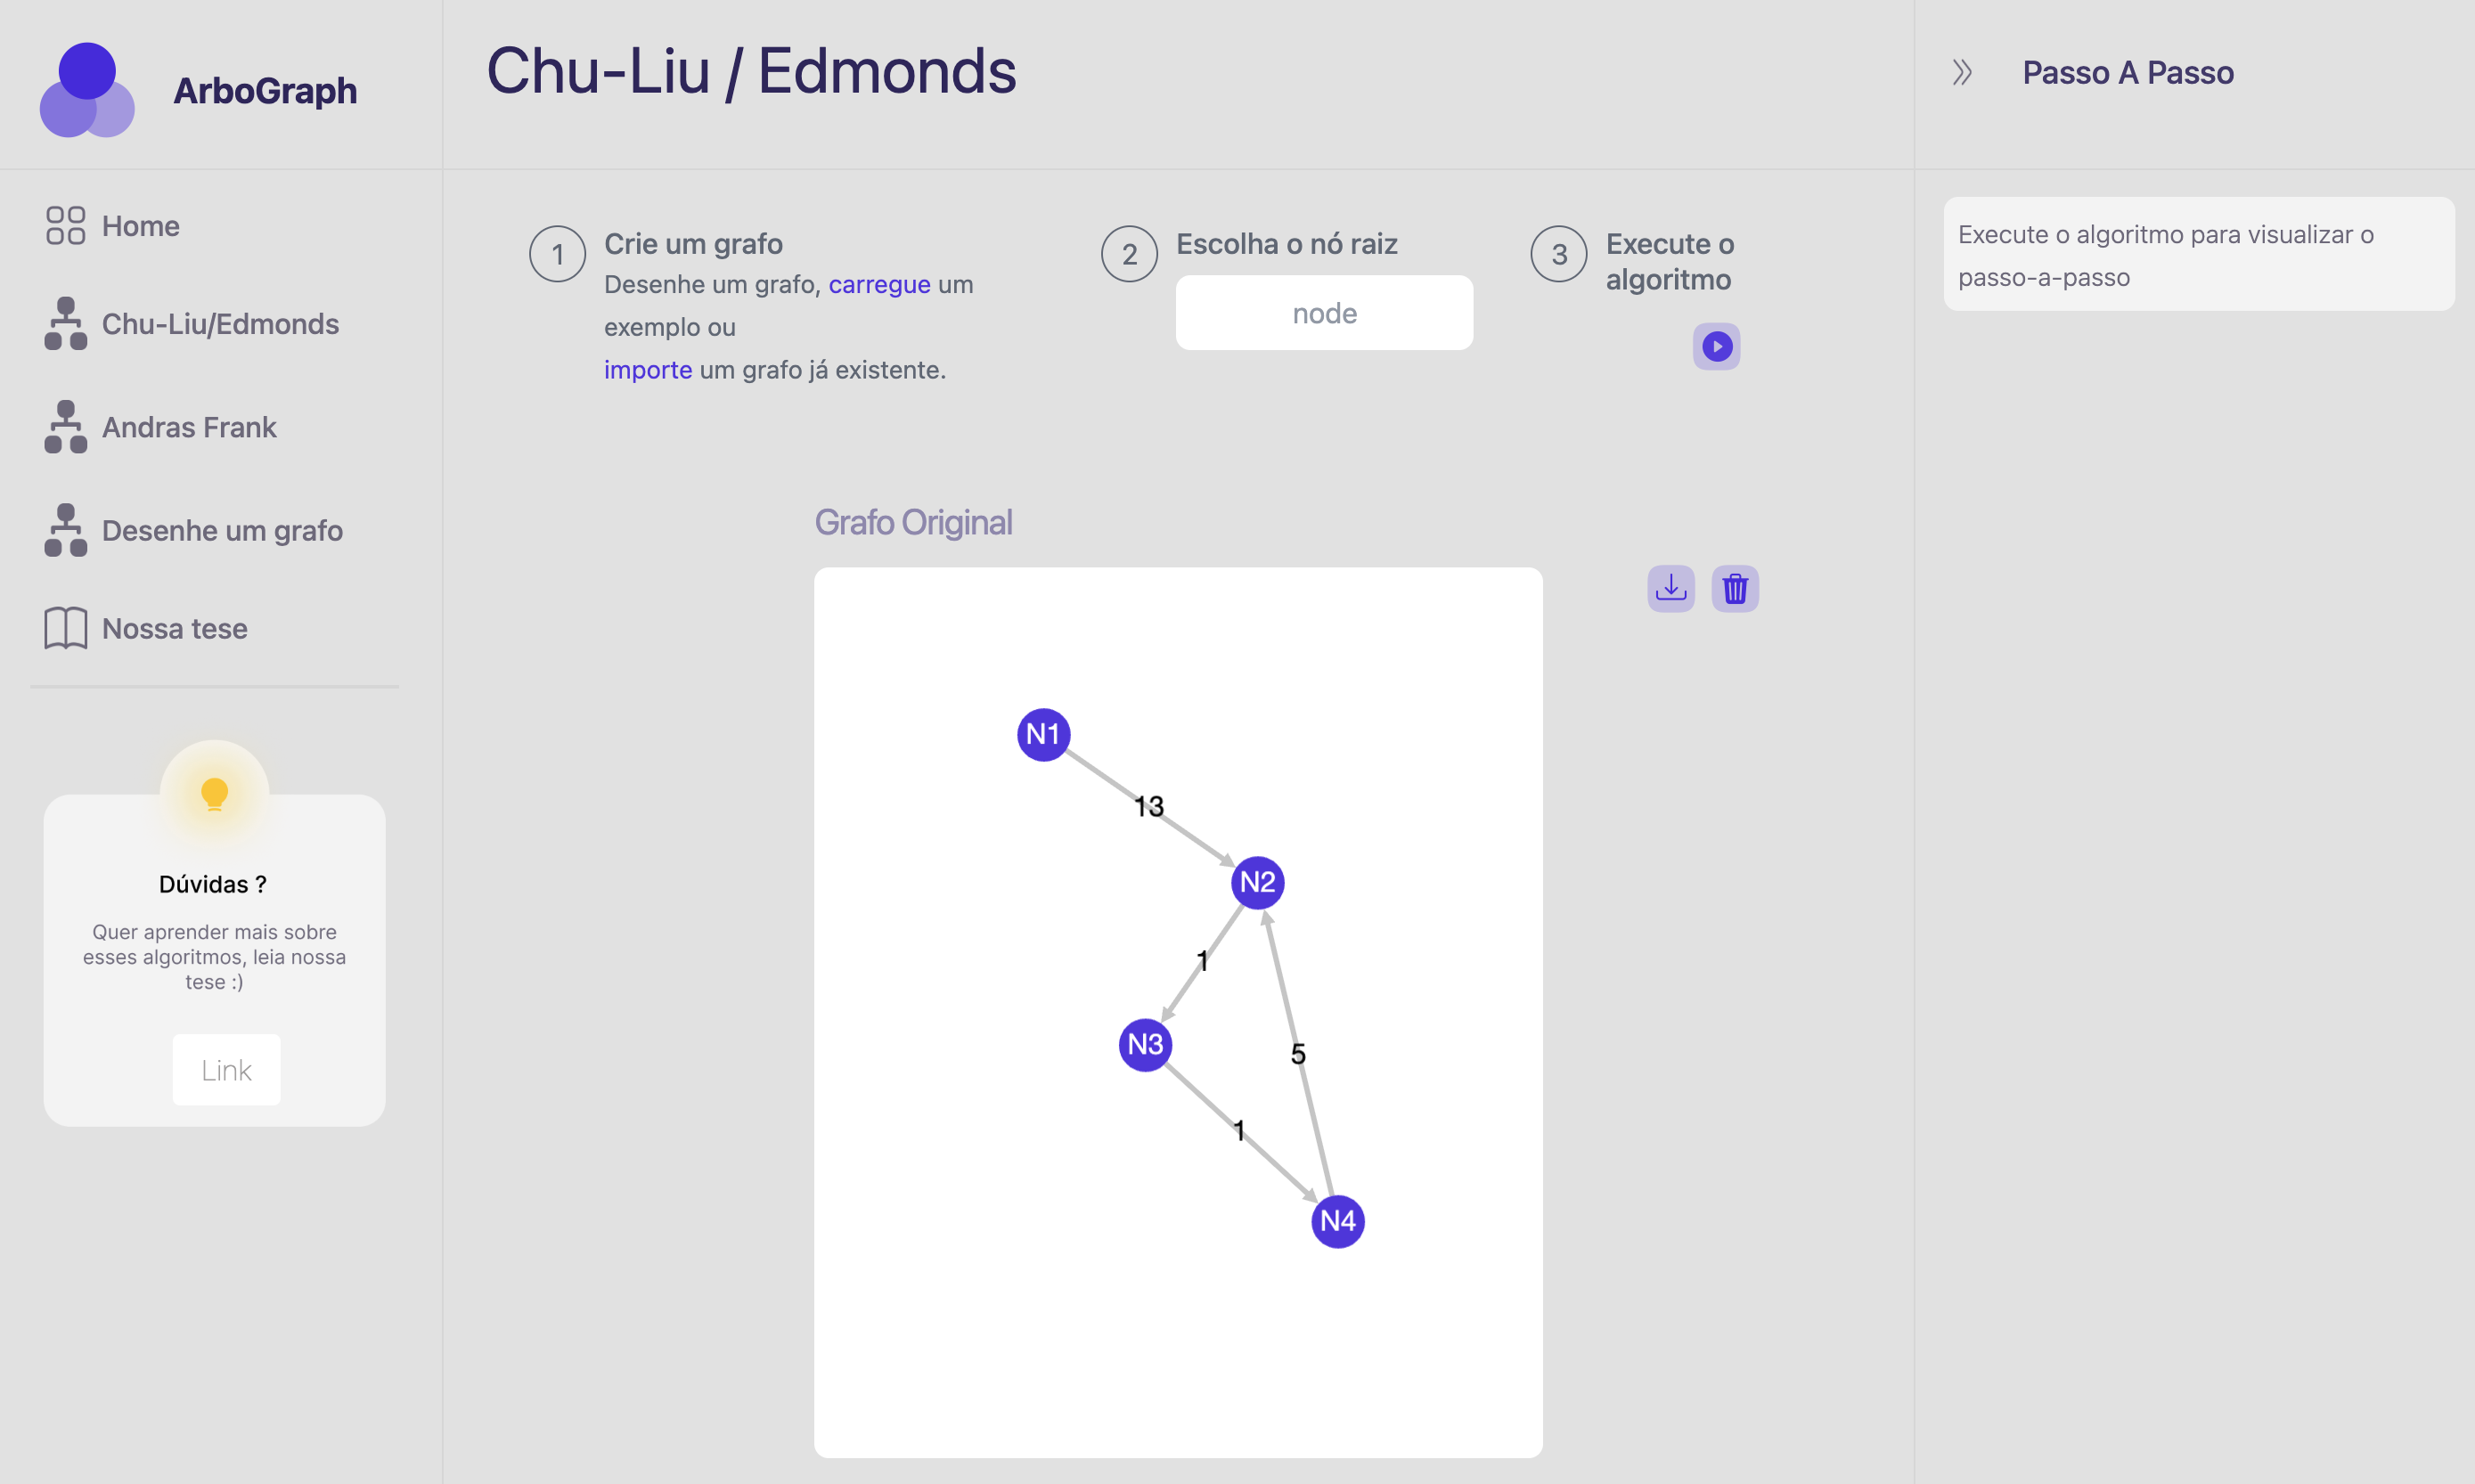
\includegraphics[width=0.95\textwidth]{../assets/chuliuhtml.png}
	\caption{Captura de tela de \texttt{chuliu.html}: criação de grafo, seleção de raiz e execução do algoritmo.}
	\label{fig:chuliu_html_screenshot}
\end{figure}

A seguir, apresentamos o código completo dessa página.

\begin{htmlbox}{chuliu.html}
	<!DOCTYPE html>
	<html lang="pt-BR">

	<head>
	<meta charset="UTF-8" />
	<meta name="viewport" content="width=device-width, initial-scale=1" />
	<title>Chu-Liu/Edmonds</title>
	<link rel="icon" type="image/x-icon" href="../assets/logo.png"/>
	<script src="https://cdn.tailwindcss.com"></script>
	<script src="https://unpkg.com/cytoscape@3.26.0/dist/cytoscape.min.js"></script>

	<link href="https://cdnjs.cloudflare.com/ajax/libs/flowbite/2.2.1/flowbite.min.css" rel="stylesheet" />
	<script src="https://cdnjs.cloudflare.com/ajax/libs/flowbite/2.2.1/flowbite.min.js"></script>

	<link rel="stylesheet" href="https://pyscript.net/releases/2025.3.1/core.css" />
	<script type="module" src="https://pyscript.net/releases/2025.3.1/core.js"></script>
	</head>

	<body class="flex min-h-screen text-gray-800 bg-gray-100">
	<style>
	.py-error, .py-terminal-error {
	display: none !important;
	}
	</style>
	<div class="absolute top-[100px] w-full h-[1px] bg-[#DBDBDB]"></div>

	<!-- MENU LATERAL -->
	<div id="sidebar"></div>

	<!-- CONTEÚDO PRINCIPAL -->
	<div id="main-content" class="flex-1 bg-[#E5E5E5] p-6">
	<span class="flex items-center gap-4 mb-10 text-4xl text-[#352B67]">Chu-Liu / Edmonds</span>
	<!-- Stepper -->
	<div class="grid grid-cols-50 gap-1">
	<div class="col-span-1 p-2">
	</div>
	<div class="col-span-9 p-2">
	<ol class="items-start gap-4 mx-4 space-y-2 sm:flex sm:space-x-4 sm:space-y-0 rtl:space-x-reverse">
	<li class="flex text-gray-500 dark:text-blue-500 space-x-2.5 rtl:space-x-reverse">
	<span class="flex items-center justify-center w-8 h-8 border border-gray-500 rounded-full shrink-0 dark:border-blue-500">
	1
	</span>
	<span>
	<h3 class="font-medium leading-tight">Crie um grafo</h3>
	<span class="text-sm text-gray-500">
	Desenhe um grafo,
	<span id="load-test-graph" class="cursor-pointer text-[#5A3CE5] hover:underline">carregue</span>
	um exemplo ou <br>
	<span id="import-graph" class="cursor-pointer text-[#5A3CE5] hover:underline">importe</span>
	<input type="file" id="file-input" style="display: none;" />
	um grafo já existente.
	</span>
	</span>
	</li>
	<li class="flex text-gray-500 dark:text-gray-400 space-x-2.5 rtl:space-x-reverse">
	<span class="flex items-center justify-center w-8 h-8 border border-gray-500 rounded-full shrink-0 dark:border-gray-400">
	2
	</span>
	<span>
	<h3 class="font-medium leading-tight">Escolha o nó raiz</h3>
	<!-- <p class="text-sm mb-2">Defina o ponto inicial</p> -->
	<input type="text" id="root-node"
	class="w-full p-2 mt-2 rounded-lg text-center focus:outline-none focus:ring-2 focus:ring-blue-500 focus:border-blue-500 border-transparent"
	placeholder="node" />
	</span>
	</li>
	<li class="flex text-gray-500 dark:text-gray-400 space-x-2.5 rtl:space-x-reverse">
	<span class="flex items-center justify-center w-8 h-8 border border-gray-500 rounded-full shrink-0 dark:border-gray-400">
	3
	</span>
	<span>
	<h3 class="font-medium leading-tight">Execute o algoritmo</h3>
	<div class="mt-1 flex justify-center items-center gap-1">
	<img id="run-algorithm" src="../assets/run.png" alt="Executar"
	class="cursor-pointer w-8 h-8 rounded-lg hover:opacity-80 mt-2" />
	</div>
	</span>
	</li>
	</ol>
	</div>
	<div class="col-span-1 p-2">
	</div>
	</div>
	<!-- Grafo original -->
	<div class="grid grid-cols-10 gap-4 py-4 px-4">
	<div class="col-span-2 p-4"></div>
	<div class="col-span-6 p-4">
	<span class="mb-50 text-xl text-[#9993B7]">Grafo Original</span>
	<div id="graph-editor" class="my-3 mt-50 py-4 px-50 rounded-lg bg-white h-[500px]">
	</div>
	</div>
	<div class="col-span-2 p-4">
	<div class="py-4 px-2 flex justify-left items-center gap-1">
	<img src="../assets/download.png" alt="Download" id="export-graph-original"
	class="my-5 cursor-pointer w-8 h-8 rounded-lg hover:opacity-80" />
	<img src="../assets/delete.png" alt="Reset" id="reset-graph"
	class="my-5 cursor-pointer w-8 h-8 rounded-lg hover:opacity-80" />
	</div>
	</div>

	</div>
	<!-- Arborescência -->
	<div id="arborescence-section" class="grid grid-cols-10 gap-4 py-4 px-4 hidden">
	<div class="col-span-2 p-4"></div>
	<div class="col-span-6 p-4">
	<span class="mb-50 text-xl text-[#9993B7]">Arborescência</span>
	<div id="arborescence-viewer" class="my-3 mt-50 py-4 px-50 rounded-lg bg-white h-[500px]">
	</div>
	</div>
	<div class="col-span-2 p-4">
	<div class="py-4 px-2 flex justify-left items-center gap-1">
	<img src="../assets/download.png" alt="Download" id="export-graph-arborescencia"
	class="my-5 cursor-pointer w-8 h-8 rounded-lg hover:opacity-80" />
	</div>
	</div>
	</div>

	<!-- Logs de execução -->
	<div id="log-section" class="grid grid-cols-10 gap-4 py-4 px-4 hidden">
	<div class="col-span-2 p-4"></div>
	<div class="col-span-6 p-4">
	<button id="collapser-button"
	class="w-full bg-[#EEEEEE] text-[#948EB3] py-2 px-4 rounded-t-md text-left flex justify-between items-center"
	onclick="toggleCollapser()">
	Log de Execução
	<img id="collapser-icon" src="../assets/plus.png" alt="Contrair" class="w-5 h-5 hover:opacity-80" />
	</button>

	<!-- Conteúdo colapsável -->
	<div id="log-collapser-content"
	class="p-4 bg-[#EEEEEE] text-sm text-gray-400 rounded-b-md hidden transition-all duration-500 ease-in-out">
	<textarea id="log-output" readonly
	class="w-full p-3 rounded h-40 bg-[#EEEEEE] text-sm text-gray-400 border-transparent"></textarea>
	</div>
	</div>
	</div>
	</div>

	<!-- Passo a Passo -->
	<div id="right-sidebar" class="w-80 transition-all duration-300 border-l-[1px] bg-[#E5E5E5] border-[#DBDBDB] overflow-hidden">
	<div id="title_step_area" class="flex items-center gap-6 py-8 mx-4 top-6">
	<button id="toggle-sidebar" class="text-right text-[#4B4277] hover:text-[#2d255d]">
	<img id="collapser-icon" src="../assets/back_arrow_right.png" alt="Contrair" class="w-5 h-5 hover:opacity-80" />
	</button>
	<span id="title_step" class="text-lg text-[#4B4277] font-medium">Passo A Passo</span>
	</div>
	<div id="container_step_by_step" class="my-6 mx-4 gap-4 py-2 px-2 bg-[#F5F5F5] rounded-lg">
	<span id="step_warning" class="text-sm font-light text-[#787486]">Execute o algoritmo para visualizar o passo-a-passo</span>
	</div>
	</div>

	<!-- Toasts -->
	<div id="toast-danger" class="hidden fixed top-5 right-5 z-50 flex items-center w-full max-w-xs p-4 mb-4 text-gray-500 bg-white rounded-lg shadow-sm dark:text-gray-400 dark:bg-gray-800 transition-opacity duration-500 opacity-100" role="alert">
	<div class="inline-flex items-center justify-center shrink-0 w-8 h-8 text-red-500 bg-red-100 rounded-lg dark:bg-red-800 dark:text-red-200">
	<!-- SVG de erro -->
	<svg class="w-5 h-5" aria-hidden="true" fill="currentColor" viewBox="0 0 20 20">
	<path d="M10 .5a9.5 9.5 0 1 0 9.5 9.5A9.51 9.51 0 0 0 10 .5Zm3.707 11.793a1 1 0 1 1-1.414 1.414L10 11.414l-2.293 2.293a1 1 0 0 1-1.414-1.414L8.586 10 6.293 7.707a1 1 0 0 1 1.414-1.414L10 8.586l2.293-2.293a1 1 0 0 1 1.414 1.414L11.414 10l2.293 2.293Z"/>
	</svg>
	<span class="sr-only">Error icon</span>
	</div>
	<div id="toast-danger-msg" class="ms-3 text-sm font-normal">Ocorreu um erro.</div>
	<button type="button" class="ms-auto -mx-1.5 -my-1.5 bg-white text-gray-400 hover:text-gray-900 rounded-lg focus:ring-2 focus:ring-gray-300 p-1.5 hover:bg-gray-100 inline-flex items-center justify-center h-8 w-8 dark:text-gray-500 dark:hover:text-white dark:bg-gray-800 dark:hover:bg-gray-700" data-dismiss-target="#toast-danger" aria-label="Close" onclick="document.getElementById('toast-danger').classList.add('hidden')">
	<span class="sr-only">Close</span>
	<svg class="w-3 h-3" aria-hidden="true" fill="none" viewBox="0 0 14 14">
	<path stroke="currentColor" stroke-linecap="round" stroke-linejoin="round" stroke-width="2" d="m1 1 6 6m0 0 6 6M7 7l6-6M7 7l-6 6"/>
	</svg>
	</button>
	</div>

	<!-- Modal de Imagem -->
	<div id="image-modal" class="fixed inset-0 z-50 flex items-center justify-center bg-black bg-opacity-80 hidden">
	<img id="image-modal-img" src="" alt="Imagem Ampliada" class="max-w-3xl max-h-[80vh] rounded-lg shadow-lg border-4 border-white">
	</div>

	<!-- Modal Loader -->
	<div id="loader-modal" class="fixed inset-0 z-50 flex items-center justify-center bg-black bg-opacity-30 hidden">
	<div class="flex flex-col items-center">
	<div class="w-16 h-16 border-4 border-[#5a3ce5] border-t-transparent border-solid rounded-full animate-spin"></div>
	<span class="mt-4 text-white text-lg">Processando...</span>
	</div>
	</div>

	<!-- Modal para peso da aresta -->
	<div id="edge-weight-modal" class="fixed inset-0 z-50 flex items-center justify-center bg-black bg-opacity-40 hidden">
	<div class="bg-white rounded-lg shadow-lg p-6 w-80">
	<h3 class="text-lg font-semibold mb-4 text-gray-800">Peso da aresta</h3>
	<input id="edge-weight-input" type="number" min="1" class="w-full p-2 border rounded mb-4 focus:outline-none focus:ring-2 focus:ring-blue-500" placeholder="Digite o peso" />
	<div class="flex justify-end gap-2">
	<button id="edge-weight-cancel" class="px-4 py-2 rounded bg-gray-200 text-gray-700 hover:bg-gray-300">Cancelar</button>
	<button id="edge-weight-ok" class="px-4 py-2 rounded bg-blue-600 text-white hover:bg-blue-700">OK</button>
	</div>
	</div>
	</div>

	<!-- Scripts -->
	<script src="../scripts/js/sidebar.js"></script>
	<script src="../scripts/js/main.js"></script>
	<script src="../scripts/js/draw_graph.js"></script>
	<script type="py" src="../scripts/chuliu_page.py" config="../scripts/pyscript.json"></script>
	</body>
	</html>
\end{htmlbox}

A figura a seguir destaca a tripartição funcional da página: navegação lateral, conteúdo interativo central e guia de passos à direita.
\begin{figure}[H]\centering
	\begin{tikzpicture}[node distance=1.4cm]
		\node[draw,rounded corners,fill=gray!10,minimum width=1.6cm] (sb4) {Barra Lateral};
		\node[draw,rounded corners,fill=blue!8,right=0.6cm of sb4,minimum width=5.2cm,minimum height=3.4cm] (maincl) {Principal (Botão de Passos + Editor + Logs)};
		\node[draw,rounded corners,fill=green!10,right=1.6cm of maincl,minimum width=2cm,minimum height=3.4cm] (rs) {Passos};
		\draw[->] (maincl.east) -- (rs.west);
	\end{tikzpicture}
	\caption{\texttt{chuliu.html} - tripartição funcional (navegação, conteúdo interativo, guia de passos).}
\end{figure}
\textit{Comentário:} a presença do passo a passo auxilia na compreensão sequencial do algoritmo.

\subsection{\texttt{Andrasfrank.html}:} página dedicada ao visualizador do algoritmo de Andras Frank. Inclui um passo a passo guiado para criar um grafo, selecionar o vértice raiz e executar o algoritmo, com feedback visual e textual. Abaixo, apresentamos uma captura de tela da página.

% Screenshot da página Andras Frank
\begin{figure}[H]\centering
	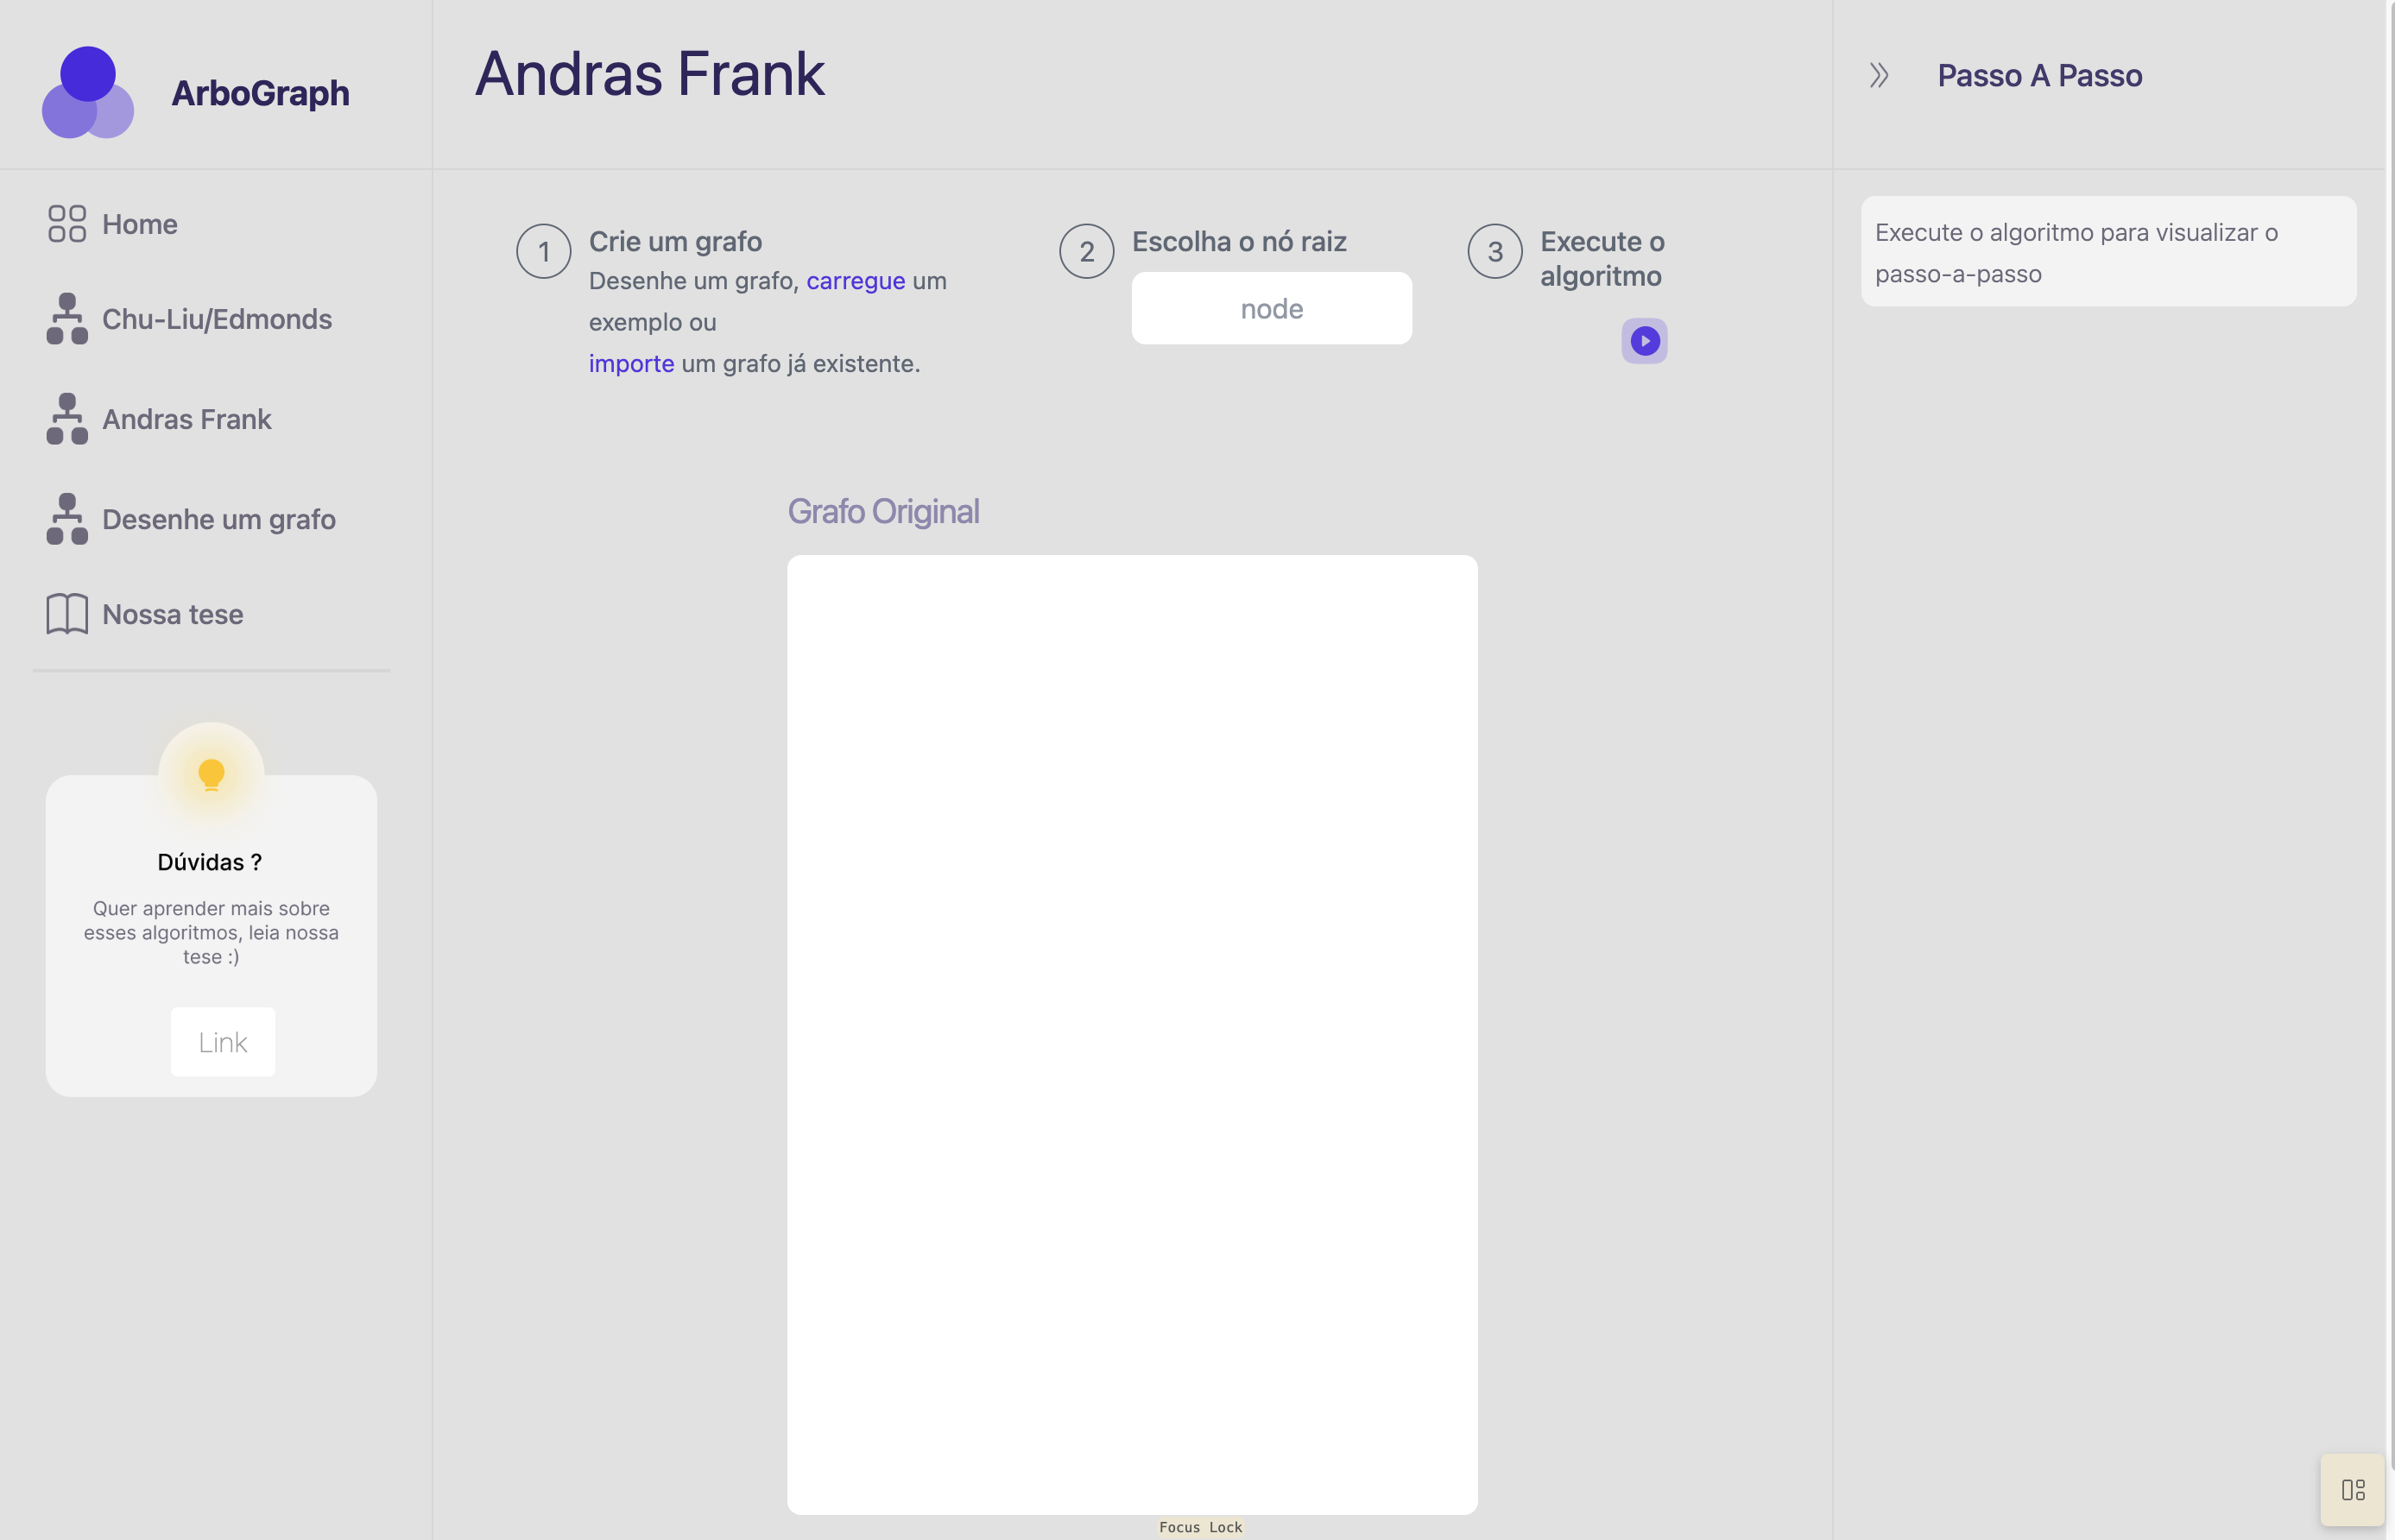
\includegraphics[width=0.95\textwidth]{../assets/andrasfrankhtml.png}
	\caption{Captura de tela de \texttt{andrasfrank.html}: interface para o procedimento em duas fases.}
	\label{fig:andrasfrank_html_screenshot}
\end{figure}

A seguir, apresentamos o código completo dessa página.

\begin{htmlbox}{andrasfrank.html}
	<!DOCTYPE html>
	<html lang="pt-BR">

	<head>
	<meta charset="UTF-8" />
	<meta name="viewport" content="width=device-width, initial-scale=1" />
	<title>Andras Frank</title>
	<link rel="icon" type="image/x-icon" href="../assets/logo.png"/>
	<script src="https://cdn.tailwindcss.com"></script>
	<script src="https://unpkg.com/cytoscape@3.26.0/dist/cytoscape.min.js"></script>

	<link href="https://cdnjs.cloudflare.com/ajax/libs/flowbite/2.2.1/flowbite.min.css" rel="stylesheet" />
	<script src="https://cdnjs.cloudflare.com/ajax/libs/flowbite/2.2.1/flowbite.min.js"></script>

	<link rel="stylesheet" href="https://pyscript.net/releases/2025.3.1/core.css" />
	<script type="module" src="https://pyscript.net/releases/2025.3.1/core.js"></script>
	</head>

	<body class="flex min-h-screen text-gray-800 bg-gray-100">
	<style>
	.py-error, .py-terminal-error {
	display: none !important;
	}
	</style>
	<div class="absolute top-[100px] w-full h-[1px] bg-[#DBDBDB]"></div>

	<!-- MENU LATERAL -->
	<div id="sidebar"></div>

	<!-- CONTEÚDO PRINCIPAL -->
	<div id="main-content" class="flex-1 bg-[#E5E5E5] p-6">
	<span class="flex items-center gap-4 mb-10 text-4xl text-[#352B67]">Andras Frank</span>

	<div class="grid grid-cols-50 gap-1">
	<div class="col-span-1 p-2">
	</div>
	<div class="col-span-9 p-2">
	<ol class="items-start gap-4 mx-4 space-y-2 sm:flex sm:space-x-4 sm:space-y-0 rtl:space-x-reverse">
	<li class="flex text-gray-500 dark:text-blue-500 space-x-2.5 rtl:space-x-reverse">
	<span class="flex items-center justify-center w-8 h-8 border border-gray-500 rounded-full shrink-0 dark:border-blue-500">
	1
	</span>
	<span>
	<h3 class="font-medium leading-tight">Crie um grafo</h3>
	<span class="text-sm text-gray-500">
	Desenhe um grafo,
	<span id="load-test-graph" class="cursor-pointer text-[#5A3CE5] hover:underline">carregue</span>
	um exemplo ou <br>
	<span id="import-graph" class="cursor-pointer text-[#5A3CE5] hover:underline">importe</span>
	<input type="file" id="file-input" style="display: none;" />
	um grafo já existente.
	</span>
	</span>
	</li>
	<li class="flex text-gray-500 dark:text-gray-400 space-x-2.5 rtl:space-x-reverse">
	<span class="flex items-center justify-center w-8 h-8 border border-gray-500 rounded-full shrink-0 dark:border-gray-400">
	2
	</span>
	<span>
	<h3 class="font-medium leading-tight">Escolha o nó raiz</h3>
	<!-- <p class="text-sm mb-2">Defina o ponto inicial</p> -->
	<input type="text" id="root-node"
	class="w-full p-2 mt-2 rounded-lg text-center focus:outline-none focus:ring-2 focus:ring-blue-500 focus:border-blue-500 border-transparent"
	placeholder="node" />
	</span>
	</li>
	<li class="flex text-gray-500 dark:text-gray-400 space-x-2.5 rtl:space-x-reverse">
	<span class="flex items-center justify-center w-8 h-8 border border-gray-500 rounded-full shrink-0 dark:border-gray-400">
	3
	</span>
	<span>
	<h3 class="font-medium leading-tight">Execute o algoritmo</h3>
	<div class="mt-1 flex justify-center items-center gap-1">
	<img id="run-algorithm" src="../assets/run.png" alt="Executar"
	class="cursor-pointer w-8 h-8 rounded-lg hover:opacity-80 mt-2" />
	</div>
	</span>
	</li>
	</ol>
	</div>
	<div class="col-span-1 p-2">
	</div>
	</div>

	<!-- Grafo original -->
	<div class="grid grid-cols-10 gap-4 py-4 px-4">
	<div class="col-span-2 p-4"></div>
	<div class="col-span-6 p-4">
	<span class="mb-50 text-xl text-[#9993B7]">Grafo Original</span>
	<div class="my-3 mt-50 py-4 px-50 rounded-lg bg-white">
	<!-- <span id="draw_warning" class="text-sm font-light text-[#787486] mx-9">Desenhe ou importe um grafo.</span> -->
	<div id="graph-editor" class="my-3 mt-50 py-4 px-50 rounded-lg bg-white h-[500px]">
	</div>
	</div>
	</div>
	<div class="col-span-2 p-4">
	<div class="py-4 px-2 flex justify-left items-center gap-1">
	<img src="../assets/download.png" alt="Download" id="export-graph-original"
	class="my-5 cursor-pointer w-8 h-8 rounded-lg hover:opacity-80 hidden" />
	</div>
	</div>

	</div>
	<!-- Arborescência -->
	<div id="arborescence-section" class="grid grid-cols-10 gap-4 py-4 px-4 hidden">
	<div class="col-span-2 p-4"></div>
	<div class="col-span-6 p-4">
	<span class="mb-50 text-xl text-[#9993B7]">Arborescência</span>
	<div id="arborescence-viewer" class="my-3 mt-50 py-4 px-50 bg-white rounded-lg h-[500px]">
	</div>
	</div>
	<div class="col-span-2 p-4">
	<div class="py-4 px-2 flex justify-left items-center gap-1">
	<img src="../assets/download.png" alt="Download" id="export-graph-arborescencia"
	class="my-5 cursor-pointer w-8 h-8 rounded-lg hover:opacity-80" />
	</div>
	</div>

	</div>

	<!-- Logs de execução -->
	<div id="log-section" class="grid grid-cols-10 gap-4 py-4 px-4 hidden">
	<div class="col-span-2 p-4"></div>
	<div class="col-span-6 p-4">
	<button id="collapser-button"
	class="w-full bg-[#EEEEEE] text-[#948EB3] py-2 px-4 rounded-t-md text-left flex justify-between items-center"
	onclick="toggleCollapser()">
	Log de Execução
	<img id="collapser-icon" src="../assets/plus.png" alt="Contrair" class="w-5 h-5 hover:opacity-80" />
	</button>

	<!-- Conteúdo colapsável -->
	<div id="log-collapser-content"
	class="p-4 bg-[#EEEEEE] text-sm text-gray-400 rounded-b-md hidden transition-all duration-500 ease-in-out">
	<textarea id="log-output" readonly
	class="w-full p-3 rounded h-40 bg-[#EEEEEE] text-sm text-gray-400 border-transparent"></textarea>
	</div>
	</div>
	</div>
	</div>

	<!-- Passo a Passo -->
	<div id="right-sidebar" class="w-80 transition-all duration-300 border-l-[1px] bg-[#E5E5E5] border-[#DBDBDB] overflow-hidden">
	<div id="title_step_area" class="flex items-center gap-6 py-8 mx-4 top-6">
	<button id="toggle-sidebar" class="text-right text-[#4B4277] hover:text-[#2d255d]">
	<img id="collapser-icon" src="../assets/back_arrow_right.png" alt="Contrair" class="w-5 h-5 hover:opacity-80" />
	</button>
	<span id="title_step" class="text-lg text-[#4B4277] font-medium">Passo A Passo</span>
	</div>
	<div id="container_step_by_step" class="my-6 mx-4 gap-4 py-2 px-2 bg-[#F5F5F5] rounded-lg">
	<span id="step_warning" class="text-sm font-light text-[#787486]">Execute o algoritmo para visualizar o passo-a-passo</span>
	</div>
	</div>

	<!-- Toast de Erro -->
	<div id="toast-danger" class="hidden fixed top-5 right-5 z-50 flex items-center w-full max-w-xs p-4 mb-4 text-gray-500 bg-white rounded-lg shadow-sm dark:text-gray-400 dark:bg-gray-800 transition-opacity duration-500 opacity-100" role="alert">
	<div class="inline-flex items-center justify-center shrink-0 w-8 h-8 text-red-500 bg-red-100 rounded-lg dark:bg-red-800 dark:text-red-200">
	<!-- SVG de erro -->
	<svg class="w-5 h-5" aria-hidden="true" fill="currentColor" viewBox="0 0 20 20">
	<path d="M10 .5a9.5 9.5 0 1 0 9.5 9.5A9.51 9.51 0 0 0 10 .5Zm3.707 11.793a1 1 0 1 1-1.414 1.414L10 11.414l-2.293 2.293a1 1 0 0 1-1.414-1.414L8.586 10 6.293 7.707a1 1 0 0 1 1.414-1.414L10 8.586l2.293-2.293a1 1 0 0 1 1.414 1.414L11.414 10l2.293 2.293Z"/>
	</svg>
	<span class="sr-only">Error icon</span>
	</div>
	<div id="toast-danger-msg" class="ms-3 text-sm font-normal">Ocorreu um erro.</div>
	<button type="button" class="ms-auto -mx-1.5 -my-1.5 bg-white text-gray-400 hover:text-gray-900 rounded-lg focus:ring-2 focus:ring-gray-300 p-1.5 hover:bg-gray-100 inline-flex items-center justify-center h-8 w-8 dark:text-gray-500 dark:hover:text-white dark:bg-gray-800 dark:hover:bg-gray-700" data-dismiss-target="#toast-danger" aria-label="Close" onclick="document.getElementById('toast-danger').classList.add('hidden')">
	<span class="sr-only">Close</span>
	<svg class="w-3 h-3" aria-hidden="true" fill="none" viewBox="0 0 14 14">
	<path stroke="currentColor" stroke-linecap="round" stroke-linejoin="round" stroke-width="2" d="m1 1 6 6m0 0 6 6M7 7l6-6M7 7l-6 6"/>
	</svg>
	</button>
	</div>

	<!-- Modal de Imagem -->
	<div id="image-modal" class="fixed inset-0 z-50 flex items-center justify-center bg-black bg-opacity-80 hidden">
	<img id="image-modal-img" src="" alt="Imagem Ampliada" class="max-w-3xl max-h-[80vh] rounded-lg shadow-lg border-4 border-white">
	</div>

	<!-- Modal Loader -->
	<div id="loader-modal" class="fixed inset-0 z-50 flex items-center justify-center bg-black bg-opacity-30 hidden">
	<div class="flex flex-col items-center">
	<div class="w-16 h-16 border-4 border-[#5a3ce5] border-t-transparent border-solid rounded-full animate-spin"></div>
	<span class="mt-4 text-white text-lg">Processando...</span>
	</div>
	</div>

	<!-- Modal para peso da aresta -->
	<div id="edge-weight-modal" class="fixed inset-0 z-50 flex items-center justify-center bg-black bg-opacity-40 hidden">
	<div class="bg-white rounded-lg shadow-lg p-6 w-80">
	<h3 class="text-lg font-semibold mb-4 text-gray-800">Peso da aresta</h3>
	<input id="edge-weight-input" type="number" min="1" class="w-full p-2 border rounded mb-4 focus:outline-none focus:ring-2 focus:ring-blue-500" placeholder="Digite o peso" />
	<div class="flex justify-end gap-2">
	<button id="edge-weight-cancel" class="px-4 py-2 rounded bg-gray-200 text-gray-700 hover:bg-gray-300">Cancelar</button>
	<button id="edge-weight-ok" class="px-4 py-2 rounded bg-blue-600 text-white hover:bg-blue-700">OK</button>
	</div>
	</div>
	</div>

	<!-- Scripts -->
	<script src="../scripts/js/sidebar.js"></script>
	<script src="../scripts/js/main.js"></script>
	<script src="../scripts/js/draw_graph.js"></script>
	<script type="py" src="../scripts/andrasfrank_page.py" config="../scripts/pyscript.json"></script>
	</body>

	</html>
\end{htmlbox}

A figura a seguir ilustra a reutilização do padrão de tripartição funcional para manter consistência cognitiva entre páginas.

\begin{figure}[H]\centering
	\begin{tikzpicture}[node distance=1.4cm]
		\node[draw,rounded corners,fill=gray!10,minimum width=1.6cm] (sb5) {Barra Lateral};
		\node[draw,rounded corners,fill=blue!8,right=0.6cm of sb5,minimum width=5.2cm,minimum height=3.4cm] (mainaf) {Principal (Passos + Editor + Logs)};
		\node[draw,rounded corners,fill=green!10,right=2.6cm of mainaf,minimum width=2cm,minimum height=3.4cm] (rsa) {Passos};
		\draw[->] (mainaf.east) -- (rsa.west);
	\end{tikzpicture}
	\caption{\texttt{andrasfrank.html} - reutilização de padrão para consistência cognitiva.}
\end{figure}
\textit{Comentário:} a consistência reduz custo de alternância ao comparar abordagens; facilita estudos controlados de diferença de entendimento.


O ecossistema de páginas cria uma narrativa pedagógica: contextualização (\texttt{home}) \,$\rightarrow$\, experimentação livre (\texttt{draw\_graph}) \,$\rightarrow$\, exploração guiada (\texttt{chuliu}, \texttt{andrasfrank}) \,$\rightarrow$\, consolidação formal (\texttt{tese}). Tal sequência segue princípios de \emph{spiral curriculum} e reduz carga intrínseca inicial.


A figura a seguir sumariza o fluxo e a reutilização arquitetural entre páginas.


\subsection{Síntese arquitetural das páginas}
\begin{figure}[H]\centering
	\begin{tikzpicture}[node distance=2.2cm,>=Stealth]
		\node[draw,rounded corners,fill=purple!10] (home) {home};
		\node[draw,rounded corners,fill=purple!10,right=of home] (draw) {draw\_graph};
		\node[draw,rounded corners,fill=purple!10,right=of draw] (ch) {chuliu};
		\node[draw,rounded corners,fill=purple!10,right=of ch] (afp) {andrasfrank};
		\node[draw,rounded corners,fill=orange!20,above=of ch] (sb) {barra lateral};
		\node[draw,rounded corners,fill=purple!20,above=of sb] (ts) {tese};
		\draw[->] (home) -- (draw);
		\draw[->] (draw) -- (ch);
		\draw[->] (ch) -- (afp);
		\draw[->] (sb) -- (ts);
		\foreach \x in {home,draw,ch,afp,ts} {\draw[->] (sb) -- (\x);}
	\end{tikzpicture}
	\caption{A \texttt{barra lateral} injeta navegação consistente; páginas de algoritmo formam trilha exploratória (instância livre \textrightarrow algoritmo 1 \textrightarrow algoritmo 2).}
\end{figure}


A arquitetura modular e reutilizável das páginas \textit{web} facilita manutenção, extensão e consistência. A barra lateral comum reduz esforço cognitivo ao navegar, enquanto o padrão tripartido de conteúdo interativo reforça familiaridade. A sequência lógica de páginas guia o usuário do contexto à experimentação e formalização, alinhando-se a princípios pedagógicos. Essa estrutura coesa apoia o aprendizado eficaz des conceitos de arborescências dirigidas e algoritmos associados.

\section{Avaliação da Interface}
\subsection{wip}
\textcolor{red}{A avaliação preliminar da interface \textit{web} envolveu testes com um grupo de usuários composto por estudantes de graduação em ciência da computação e profissionais da área. Os participantes foram convidados a utilizar o visualizador interativo para criar grafos, executar os algoritmos de Chu-Liu/Edmonds e Andras Frank, e explorar os passos detalhados. Feedback qualitativo foi coletado através de questionários e entrevistas, focando na usabilidade, clareza das instruções, eficácia do passo a passo e compreensão dos algoritmos.}

\subsubsection{wip}
\textcolor{red}{Os resultados indicaram que a maioria dos usuários considerou a interface intuitiva e fácil de navegar. O passo a passo foi particularmente elogiado por facilitar a compreensão dos algoritmos, permitindo que os usuários acompanhassem cada etapa do processo. Alguns participantes sugeriram melhorias, como a inclusão de mais exemplos de grafos e a possibilidade de salvar e carregar sessões de trabalho.}

\section{Comentários finais sobre a Interface \textit{web}}
Este capítulo detalhou a implementação técnica do visualizador interativo de arborescências dirigidas, cobrindo desde a arquitetura \textit{web} até a integração de algoritmos complexos. A escolha de tecnologias modernas como HTML5, CSS3, JavaScript e PyScript permitiu criar uma interface intuitiva e responsiva, facilitando a experimentação e compreensão dos algoritmos de Chu-Liu/Edmonds e Andras Frank. A reutilização de padrões arquiteturais entre páginas promoveu consistência cognitiva, enquanto a estrutura modular facilitou manutenção e extensão futura. A avaliação preliminar indica que a ferramenta atende aos objetivos pedagógicos, embora melhorias possam ser feitas com base no feedback dos usuários. No próximo capítulo, discutiremos as considerações finais e perspectivas futuras para o projeto.
